\documentclass[11pt,a4paper,titlepage,oneside]{report}
\usepackage{titling}
\usepackage{graphicx}
\usepackage{mathtools}
\usepackage{lmodern}
\usepackage{amsmath}
\usepackage{float}
\usepackage{subfig}
\usepackage{listings}
\usepackage[hidelinks]{hyperref}
\usepackage{url}
\usepackage[backend=biber]{biblatex}
\usepackage{makecell}

\addbibresource{bibtex.bib}

%% Memoir layout setup

%% NOTE: You are strongly advised not to change any of them unless you
%% know what you are doing.  These settings strongly interact in the
%% final look of the document.

% Dependencies
\usepackage{bfhlogo}
\usepackage{etoolbox}% http://ctan.org/pkg/etoolbox

\makeatletter
%%begin novalidate
%% Titlepage adjustments
\pretitle{\vspace{0pt plus 0.7fill}\begin{center}\Huge}
\posttitle{\end{center}\par}
\preauthor{\par\begin{center}\let\and\\\Large}
\postauthor{\end{center}}
\predate{\par\begin{center}\Large}
\postdate{\end{center}}
%%end novalidate
\def\@advisors{}
\newcommand{\advisors}[1]{\def\@advisors{#1}}
\def\@department{}
\newcommand{\department}[1]{\def\@department{#1}}
\def\@thesistype{}
\newcommand{\thesistype}[1]{\def\@thesistype{#1}}

\renewcommand{\maketitlehooka}{\noindent\bfhlogo[2cm]}

\renewcommand{\maketitlehookb}{\vspace{1in}%
  \par\begin{center}\Large\sffamily\@thesistype\end{center}}

\renewcommand{\maketitlehookd}{%
  \vfill\par
  \begin{flushright}
    \sffamily
    \@advisors\par
    \@department, BFH
  \end{flushright}
}

% Fix the chapters (unnecessary space)
\patchcmd{\@makechapterhead}{\vspace*{50\p@}}{}{}{}% Removes space above \chapter head
\patchcmd{\@makeschapterhead}{\vspace*{50\p@}}{}{}{}% Removes space above \chapter* head

\makeatother

\setlength{\droptitle}{-48pt}


\setlength{\parindent}{0pt}

\title{Open source SLAM library for embedded systems}
\author{Stefan Eichenberger\\<eichest@gmail.com>}
\date{January 2020}
\advisor{Prof. Marcus Hudritsch}
\expert{Dr. Harald Studer (Optimo Medical AG)}
\department{TSM CPVR Lab}

\lstset{
  basicstyle=\ttfamily\scriptsize
}

\begin{document}

\maketitle
\begin{abstract}
	Simultaneous location and mapping (SLAM) is a technology used for robot navigation and augmented reality. Today most SLAM libraries are proprietary or not ready for embedded systems. In this thesis, we will write and analyse a library which is open source and is usable on embedded devices.
\end{abstract}

\section*{Executive Summary}
Today we use Simultaneous Location and Mapping (SLAM) for robot navigation and augmented reality. Often this algorithms need a high performance graphics card or a high performance processor. For industrial and robotics purposes we have constraints in space, temperature and power consumption. Therefore, we require devices with less power consuming CPUs which are also less powerful. In this thesis we implement and analyse an algorithm called SVO which the authors claim is capable to run on embedded devices. The reference implementation uses monocular cameras, while we use a stereo camera. We show that the algorithm is based on optical flow which is a well-known principle in computer vision. The implemented algorithm performs 4 tasks. It maintains a 3D point cloud which is used to guess the camera pose. Then it does a pose estimation based on the 3D cloud which first estimates the pose. We call this sparse image alignment and it uses a changed version of optical flow which directly outputs a pose instead of a warp matrix. To make the guess more accurate it, then refines the pose by using standard optical flow followed by a minimization of the re-projection error. In a last step the algorithm performs a 3D point cloud update where we refine the cloud by taking the new pose into account.\\
We show that the algorithm works as described and can estimate the 3D pose as described by the authors of SVO. We see that the algorithm performs faster than a comparable SLAM algorithm called ORB SLAM. However, the current implementation is less accurate than ORB. We conclude that SVO shows great promise as a SLAM algorithm for embedded devices. However, the current implementation is not production ready and would need improvements.

\tableofcontents

\chapter{Introduction}

Humans use different sensors to estimate the pose of the head inside a room. Everyone ever tried to stand on one foot and closed the eyes knows that closing eyes makes finding the balance harder. From this we can guess that our eyes are an import factor for finding the pose for our brain. In this thesis we try to use the same optical information from a camera to estimate the angle and position (pose) relative to the first image. We call this visual odometry (VO). Most algorithms that implement visual odometry also require SLAM (Simultaneous Localization and Mapping). Such algorithms create a map of the environment while constantly estimating the camera pose. Therefore, we use this term interchangeably in this document. Knowing the position of an object is important in a lot of different applications and becomes more and more important towards autonomous navigation. Examples of such applications are e.g. drone navigation, robot navigation or augmented reality. The listed applications require a flexible and ideally mobile device. Therefore, we can’t use a PC with a huge power supply. So such an algorithm should ideally be able to run on embedded devices without the requirement of having powerful GPUs or CPUs available.\\
The CPVR lab at the Bern university of applied science uses an algorithm called ORB SLAM \cite{orbslam} for projects related to augmented reality. They could tweak the algorithm to achieve an acceptable frame rate of 10-20 frames per second(fps) on mobile phones. However, a faster frame rate would mean that no interpolation is needed or the algorithm could run on lower end devices. Therefore, we test a different algorithm for the SLAM problem in this document which is called Semi-Dens Visual Odometry (SVO) \cite{svo}. The second SVO paper \cite{svo2} from the same author states that the duration to process one frame on a modern processor is below 5ms when running on two CPUs. Even thought SVO SLAM is open source, the reference implementation is over 4 years old and has tons of 3th party dependencies. There is a newer version available based on the second paper but this implementation is closed source. However, it is based on the original idea of SVO. In this document we describe our own implementation of the SVO algorithm but we focus on stereo camera SLAM, while the original implementation uses monocular cameras. We analyse the robustness of SVO and how suitable it is to run on an embedded system which we can use for mobile applications.

\section{SLAM}

SLAM is a technology that takes images as input and generates a map of its environment while simultaneous estimating the pose of the camera. There are two groups of SLAM algorithms. Indirect SLAM algorithms extract features from an image and then try to match this feature based on descriptors with each other. For each image it is necessary to detect features, extract descriptors, compare the descriptors to previous images and then do a triangulation. On the other side, there are direct SLAM algorithms. These algorithms directly match one frame to another by its intensity differences. They optimize the pose and try to minimize the intensity difference over the whole image (dense) or at some sparse points (sparse). Figure \ref{fig:slammodes} shows an overview of the different SLAM types.

\begin{figure}[H]
  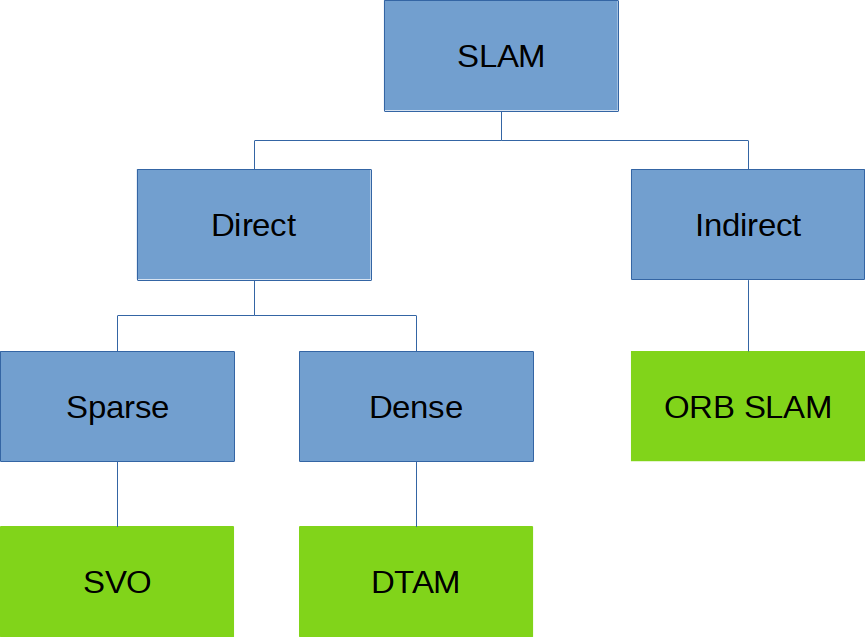
\includegraphics[width=1.0\textwidth]{img/slam_modes.png}
  \caption{SLAM Types}\label{fig:slammodes}
\end{figure}

As mentioned before we implement an SVO like algorithm during this thesis. It is part of the direct sparse group.

\section{Stereo and Monocular SLAM}

In this thesis we focus on stereo SLAM. A lot of today's paper focus on monocular SLAM. The reasons is that monocular cameras are cheaper and they are available in Smartphones. Monocular SLAM has two problems that we don’t have with stereo SLAM. First an initialization process has to estimate the movement between two frames. We can only create a 3D point cloud based on two images with known position, in the monocular case the position of two images is random. Therefore, the algorithm needs to guess the pose and transformation over a few images until it knows the poses. It does that by making assumptions on the world or by trying to optimizing the point positions over several images. However, even when successfully initialized the second problem persists. Monocular SLAM cannot to guess the scale of the point cloud. The intuition for this issue is that we can’t distinguish between the movement of the camera on a small model close to the scene or the movement of the camera on the original model further away from the scene. With stereo SLAM we don’t have this issue. For each camera pose we get two images with a known distance between the two camera sensors (baseline). Therefore, we can calculate the depth of each pixel in real world distance. From this we can generate a point cloud assuming that the initial camera pose is at origin. We therefore have an instantaneous initialization and can calculate the real world position in a known unit e.g. meters. Tracking between two camera poses is however the same on monocular and stereo SLAM. However we can again insert new keypoints immediately on stereo cameras without the need of using a second camera pose.

\section{Camera}

To do stereo computer vision, we need a stereo camera. There are a few stereo cameras available on the market. It is also possible to build a stereo camera with two monocular cameras. However, we decide against that because it would require a mechanism to synchronize the images from both streams. We analyze three stereo cameras available on the market. An ideal camera would have a high frame rate, a high resolution, a global shutter, USB3.0 with UVC driver and a high baseline (distance of the two cameras) while being cheap. Table \ref{tab:cameras} shows a comparison of a ZED camera from Stereolabs \cite{zed}, a Tara from Econ \cite{tara} and a Realsense D435 from Intel \cite{realsense}.

\tiny
\begin{table}[H]
  \centering
  \begin{tabular}{|c|c|c|c|c|c|c|c|}
  Camera & Resolution & FPS & Shutter & Driver & Baseline & IMU & Price \\
  \hline
  ZED & 1920x1080 & 30 & rolling &  UVC & 120mm & 6DoF & 449\\
  Tara & 752x480& 60 & global &  UVC &  60mm & 6DoF & 149\\
  D435 & 1280x720& 90 & global & UVC &  50mm & 6DoF & 179\\
\end{tabular}
\caption{Tested Camera Types}
\label{tab:cameras}
\end{table}
\normalsize

\begin{figure}[H]
  \centering
  \subfloat[Stereolabs ZED]{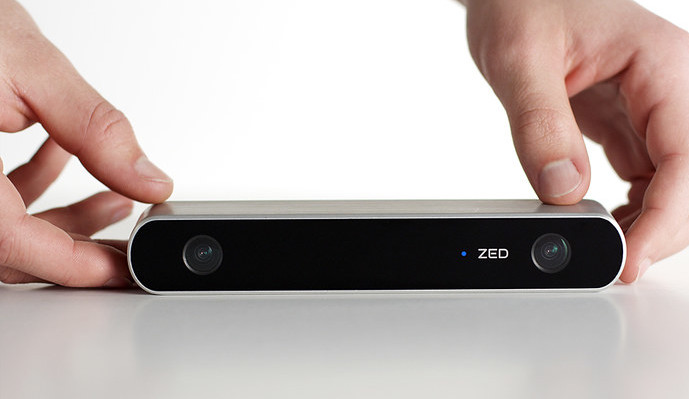
\includegraphics[width=0.3\textwidth]{img/zed_cam.jpg}}
  \subfloat[Econ Tara]{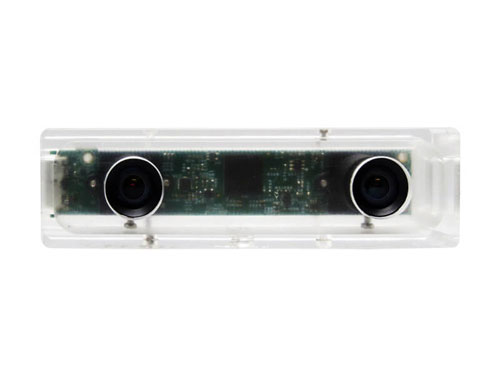
\includegraphics[width=0.3\textwidth]{img/tara_cam.jpg}}
  \subfloat[Intel Realsense D435]{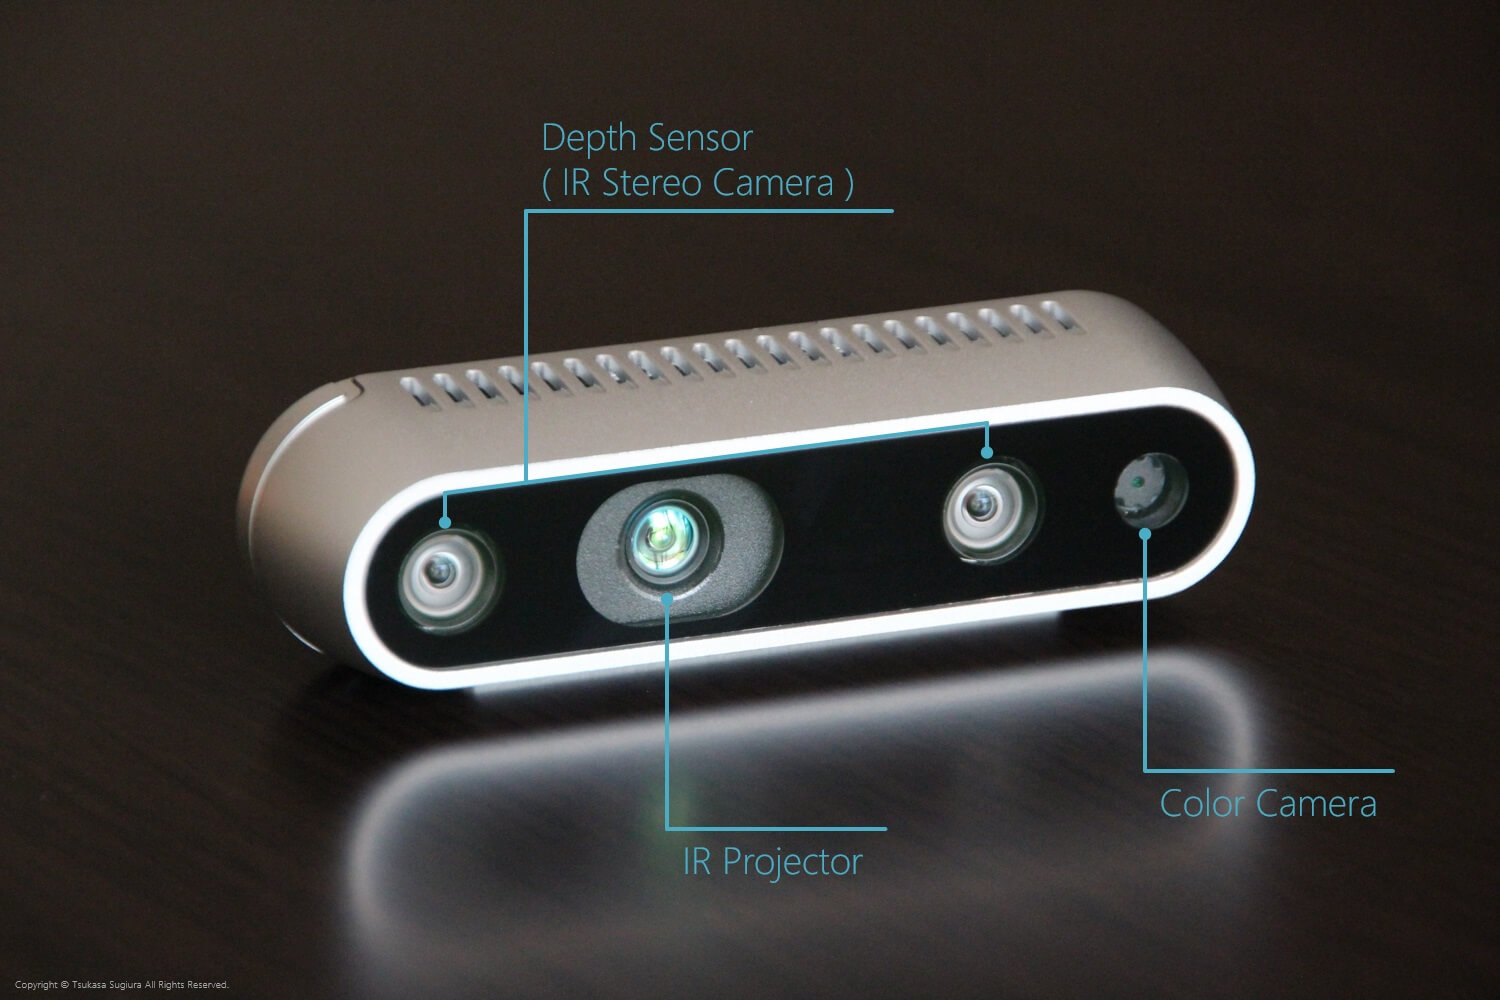
\includegraphics[width=0.3\textwidth]{img/d435_cam.jpg}}
  \caption{Tested Stereo Cameras}\label{fig:cameras}
\end{figure}


We use the Econ Tara because it has an outstanding price ratio and because it is a conventional stereo camera. However, the Intel RealSense camera is also a great fit because it delivers depth images directly. This reduces the CPU load on the iMX8. If we require Full HD, we should use the ZED camera. Another advantage of the ZED camera is the bigger baseline of 120mm. This allows depth estimation with a bigger range. We decide against this camera mainly because of the high price. We can't profit of the Full HD sensors because embedded systems only have limited CPU resources.

\section{Purpose of this Thesis}

This thesis implements SVO SLAM as open source library. Based on this implementation we do an evaluation on how well the algorithm is suited for embedded systems. We finally benchmark the implementation against the open source reference implementation regarding speed and accuracy. Further more we will provide a 3D viewer and a demo application which shows the possibilities of the SLAM library.

\section{Outline}

This document is organised as follows. We describe the SVO algorithm in chapter \ref{ch:svo}. However, we don't describe the mathematical details in depth because to not keep the chapter smaller. Chapter \ref{ch:depth} will describe how we receive depth information from a stereo camera. In chapter \ref{ch:opt_flow} we describe optical flow. We first start with an intuitive section and then move forward to the mathematical details. In chapter \ref{ch:pose_refinement} we find the information about how we can refine the pose after a first estimate. The details about how we implement the algorithm is the subject of chapter \ref{ch:implementation}. We then compare the results of the implementation with previous work in chapter \ref{ch:results}. In the last chapter \ref{ch:discussion} we discuss the final results.

\section{Planing}
The master thesis is honored with 27 ECTS. 1 ECTS consumes 30h which results in 810h. Assuming 8.5 working hours per day, we have to spend 95.29 working days. Because the thesis is done part time, we can use a full year. We assume one year has 48 weeks. During the first 16 weeks we can only spend 1.5 days for the thesis (because of additional modules). This means during the first 16 weeks we only work 24 days on the project. 71.29 days are left for the last 32 weeks. This results in 2.228 days work during the 32 weeks. Figure \ref{fig:gantt} shows the initial and the final planning. Unfortunately, implementing of the library took more time than expected. Therefore, the plane detection and mesh creation has been removed. If this is a requirement an additional library like the open source project Point Cloud Library \cite{pcl} could be used.

\begin{figure}[H]
  \subfloat[Inital planing]{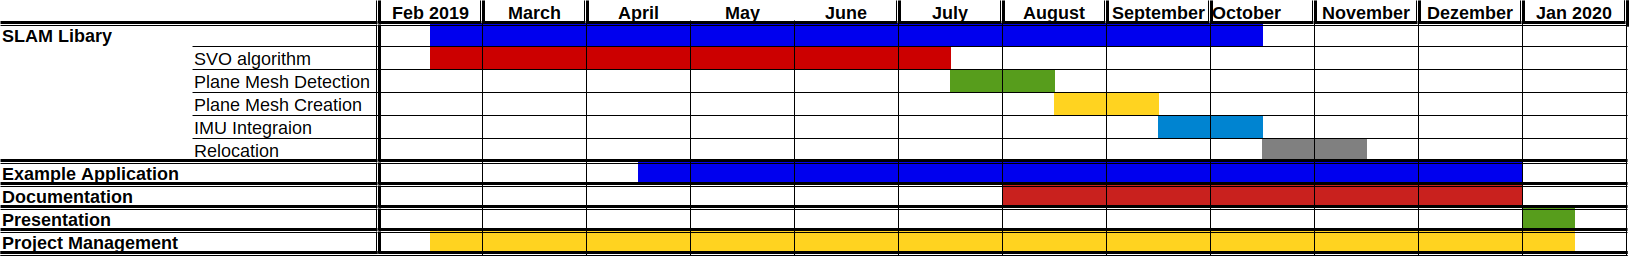
\includegraphics[width=1.0\textwidth]{img/gantt_orig.png}}\\
  \subfloat[Final planing]{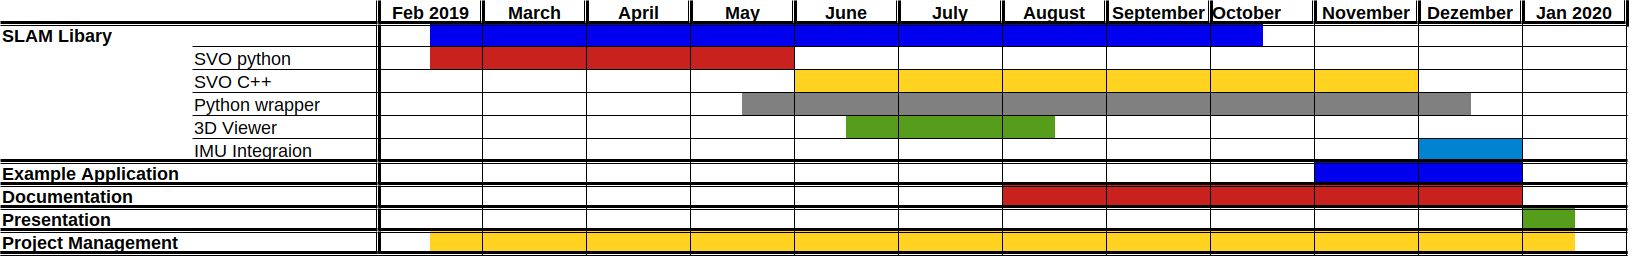
\includegraphics[width=1.0\textwidth]{img/gantt_final.png}}
  \caption{Planing}\label{fig:gantt}
\end{figure}

As the final planning shows we first started with a Python based implementation of the algorithm. The idea was that Python code is more readable and better suited for experimenting. However, the problem was that the code was slow even when using Numpy to speed up matrix multiplications. Therefore, we implemented the library completely in C++. However, for debugging a Python wrapper was developed in parallel. Reviewing this decision, this was a mistake because we spent a lot of time for debugging the Python wrapper. The final version still provides the wrapper. However, it is tested poorly and not documented.\\
Initially there was no plan to write a 3D viewer. However, to make it more flexible we developed a viewer which can receive data over Network to keep the code base separated and to allow remote analysis of 3D data. Because of this two issues and changes we reduced the scope, and we set the focus to the library.

\chapter{SVO}\label{ch:svo}
The subject of this chapter is the basic idea behind SVO SLAM. We don't dive into the mathematical details yet. As we will see most parts of the algorithm are based on the idea of optical flow. Therefore, we will handle this topic in chapter \ref{ch:opt_flow}.

\section{Architecture}

Figure \ref{fig:svo_slam} shows the architecture of SVO and our implementation. In this figure we see a lot of differences between the original implementation and what we do. However, the two main steps which are sparse model based image alignment and pose refinement are the same. Our implementation does not use multi-threading so everything is done sequential. This may surprise but has the advantage of not having to synchronize and is also more deterministic. However, it's not the whole truth. Some parts of the code are prepared to use OpenMP for multiprocessing. The idea is that the main steps are executed sequential but they use the features of multi-core processors just for each step. Using this approach we hope to spread the load more equally over all processors on modern systems instead of using separate tasks which may not scale. Further, because we focus on stereo cameras the mapping task is not required in the same depth as in SVO. We will describe this differences in a later section.

\begin{figure}[H]
  \centering
  \subfloat[Original SVO]{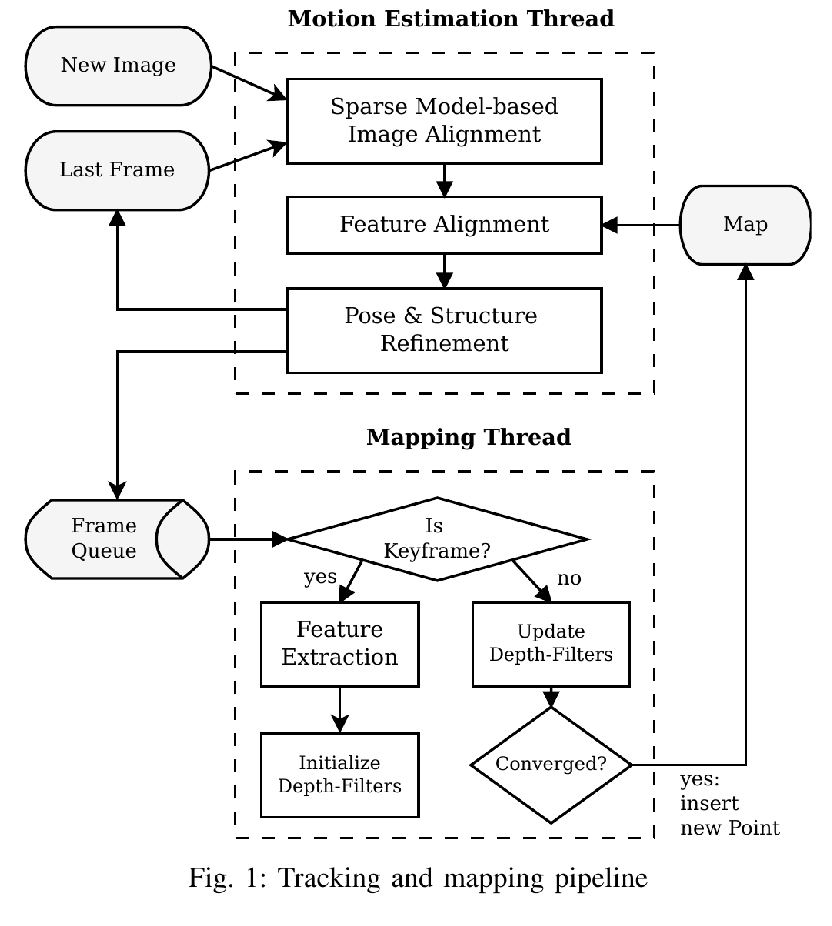
\includegraphics[height=0.25\textheight]{img/svo1_flow.png}}
	\qquad
  \subfloat[Our SVO]{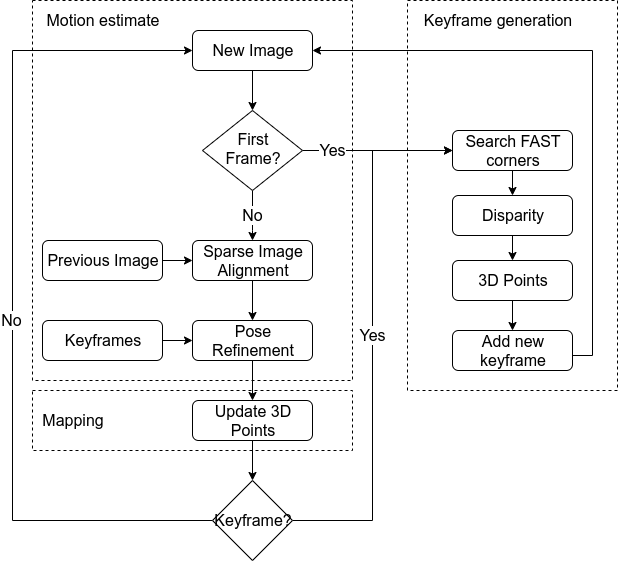
\includegraphics[height=0.25\textheight]{img/our_svo_slam.png}}
  \caption{Orignal SVO SLAM vs modified version}\label{fig:svo_slam}
\end{figure}

\section{Keyframe Generation}\label{sec:initialization}
The original SVO implementation uses a monocular camera. It's therefore not possible to estimate depth in the first picture. There must be a movement that the algorithm can estimate the depth of keypoints. However, in this thesis we use a stereo camera with a known baseline. Therefore, we can estimate the depth of a keepoint from the first image. To generate a new keyframe we perform the following steps:
\begin{enumerate}
  \item{Search FAST keypoints in the image \cite{fast}}
  \item{Do Sobel filtering of the image in horizontal direction}
  \item{Divide image in 16x16 blocks}
  \item{Select one FAST corner in each block}
		\begin{enumerate}
			\item{If no FAST corner can be found, use point with biggest gradient as keypoint}
		\end{enumerate}
  \item{Calculate depth for each keypoint}
  \item{Transform the keypoint depth to world coordinates by using the camera pose}
\end{enumerate}

The mathematical details on how to calculate the depth and the world coordinates from a stereo camera is described in chapter \ref{ch:depth}.

\section{Sparse Image Alignment}\label{sec:sia}

From the keyframe generation step we get an initial point cloud. We use this point cloud to estimate the pose and motion of the camera. We try to find a Pose that minimizes the photometric error of small patches around the keypoints. We do this by minimizing the formula shown in equation \ref{eq:intensity}. We use equation \ref{eq:camera_model} to project the 3D point cloud to the current frame. By using Gradient Descent we can minimize the intensity difference by changing the values of the extrinsic matrix $r_{ij}$ and $t_{x,y,z}$. As initial guess for the pose we use the current pose and add the motion model. The motion model is the difference between the pose in the previous frame ($t-1$) and frame $t-2$. If we have an additional IMU available we can also improve the motion model by adding information from this sensor (e.g. angle velocity).

\begin{equation}\label{eq:camera_model}
  \begin{gathered}
    \begin{pmatrix}
      u\\
      v\\
      s
    \end{pmatrix}=
    \begin{pmatrix}
      f_x & 0 & c_x \\
      0 & f_y & c_y \\
      0 & 0 & 1
    \end{pmatrix}
    \begin{pmatrix}
      r_{11} & r_{12} & r_{13} & t_x\\
      r_{21} & r_{22} & r_{23} & t_y\\
      r_{31} & r_{32} & r_{33} & t_z\\
    \end{pmatrix}
    \begin{pmatrix}
      X\\
      Y\\
      Z\\
      1
    \end{pmatrix}\\
    \begin{pmatrix}
      x\\
      y
    \end{pmatrix}=
    \begin{pmatrix}
      \frac{u}{s}\\
      \frac{v}{s}
    \end{pmatrix}
  \end{gathered}
\end{equation}
\begin{align*}
  f_x,f_y  &:  \text{Focal length}\\
  c_x,c_y  &:  \text{Principal point (z axis of camera goes through)}\\
  X,Y,Z     &: \text{Point coordinates with Camera 0,0,0}\\
  u,v,s     &: \text{Image coordinates with scale s}\\
  x,y       &: \text{Keypoint projection from 3D cloud}\\
  r_{ij}    &: \text{Camera rotation matrix}\\
  t_{x,y,z} &: \text{Camera location}
\end{align*}

\begin{equation}\label{eq:intensity}
  \sum_n\sum_x\sum_y(I_{k-1}(x'',y'')-I_{k}(x',y'))^2
\end{equation}
\begin{align*}
  x'',y''        &: \text{Warped pixel position in the template}\\
  x',y'          &: \text{Pixel position in the current image}\\
  I_{k-1}        &: \text{Template image}\\
  I_{k}          &: \text{Current image}\\
  n              &: \text{Over all keypoints}  
\end{align*}

The SVO paper \cite{svo2} describes this step in section IV.A. By performing the sparse image alignment we get a first estimate of the pose. However, because we estimate the current pose by using the previous frame we will get a drift in the long term. Therefore, we need to refine the pose by using the keyframe as reference. This is what we describe in the next section. Section \ref{sec:pose_estimation} will describe the mathematical details on how this optimization works.

\section{Pose Refinement}\label{sec:refinement}

The refinement step is necessary to reduce the drift over time by using the keyframe where a keypoint has first been seen. First we use the inverse compositional Lucas Kanade algorithm to find the new position of the point in the current image. By using the pose of the sparse image alignment we can already get an estimate of the position by doing a projection of the 3D cloud to the current image. Then we use optical flow to get a more accurate point position. We mark points that move more than 3 pixels as outliers because the sparse image alignment and the projection step should already be more accurate. We then optimize the pose so that the reprojection of the 3D point gets minimal (equation \ref{eq:refinement_problem}.

\begin{equation}\label{eq:refinement_problem}
  minimize(\sum_n ((x'-x)^2+(y'-y)^2))
\end{equation}
\begin{align*}
  x',y'   &: \text{Keypoint position found by optical flow}\\
  x,y     &: \text{Keypoint projection from 3D cloud with camera pose see \ref{eq:camera_model}}
\end{align*}

Chapter \ref{ch:opt_flow} describes optical flow and Lucas Kanade in more details. Chapter \ref{ch:pose_refinement} describes how we can calculate the gradient for minimizing the reprojection error in equation \ref{eq:refinement_problem}.

\section{Keyframe insertion}
If less than 75\% of the keypoints are tracable we need to insert a new keyframe based on the previous frame. In comparison SVO inserts a new keyframe if the movement is more than 12\% of the average depth. In a first step we try to do it as described, however maybe this needs to change in the future. See \cite{svo2} section X.D for the implementation details.

\section{Update 3D Points}

The update of the 3D points is completely different from what SVO \cite{svo} does. The reason is that we can measure the keypoint depth in the first frame by using the stereo images. SVO uses a bayesian filter approach to estimate the keypoint depth over time. We instead use a mechanism to detect outliers and a simple Kalman Filter to update the 3D position of 3D keypoints.

\subsection{Outlier detection}
The outlier detection has two steps. During refinement the intensity difference returned by optical flow is checked. If it exceeds an empirically determined value of 20 it will mark the point as outlier. This can happen if points get occluded by objects and are therefore not visible in the new image anymore. Another mechanism that doesn't mark a point as outlier but masks it during refinement is if a point moves more than 9pixels. This can happen if there is low texture at the keypoint and it moves therefore more than expected. However, such points can still help to improve the position during sparse image alignment.\\
A second mechanism to detect outliers is used before point refinement. The mechanism calculates does a depth estimation with the current image and then checks if the new estimated 3D point near the previous estimated 3D point. It uses the variance of 0.5 pixel and transfers this into a difference in point location. If the previous estimated 3D point is within the current estimate +- 5 Tau the point is assumed as inlier. If it's not within this estimate it's estimated as outlier. We count the inlier and outlier. If we see more outlier than inlier for one keypoint we remove it from the list of available keypoints. This helps us to detect points that have a bad estimate or are in areas with low texture.

\subsection{Point Refinement}
As we saw before SVO \cite{svo} uses monocular cameras. For that it is necessary to have multiple images at multiple positions to get a initial guess of the 3D cloud. The algorithm initializes each keypoint with an average depth, estimates the new pose based on this depths and updates the depth based on the new pose. The keypoints are first threaded as seeds and only if the certainty of the depth is high enough the point is added into the 3D map. The whole 3D point estimation only works if there is movement in x or y direction and for the first n frames there is no point cloud available. Because we use a stereo camera we are not affected by that (as we saw in section \ref{sec:initialization}). However, we can improve the position of a 3D point over time. In section \ref{sec:refinement} we got a better estimate of the keypoint location in the current image by using optical flow. We then refined the pose based on this information. However, because the 3D points are 100\% accurate we still have some error between the point found by optical flow and the point from the reprojection. If the camera moved more than the baseline of the camera we may profit from this movement to get a better estimate of the 3D position. We do this by using a Kalman filter with the update step shown in equation \ref{eq:point_refinement}. The measurement error is smaller the bigger the movement is. For the first measurement we know that the disparity has the size of the baseline of the camera. This means instead of $\sqrt{\Delta x^2+\Delta y^2}$ we just take the baseline in meter. Only the disparity has an approximate normal distribution. Therefore we can't predict the depth but the inverse depth based on the current measurement. This is why we use $z^{-1}$ in the formula.
\begin{equation}\label{eq:point_refinement}
  \begin{gathered}
    z^{-1}(t)=z(t-1)+w(t)\\
    y(t)=z^{-1}(t)+v(t)\\
    w(t)=0.01\\
    v(t)=\frac{0.5}{\sqrt{\Delta x^2 + \Delta y^2}}
  \end{gathered}
\end{equation}
\begin{align*}
  \Delta x, \Delta y  &: \text{Movement of the camera}\\
  w                   &: \text{New information}\\
  v                   &: \text{Measurement error/noise}\\
\end{align*}

\chapter{Depth Estimation}\label{ch:depth}

To find the depth at a certain point (.e.g. keypoint) we match the intensities of the left and right images for a certain patch. Because we vertically aligned the camera, the algorithm starts matching the right image at pixel position of the left image and searches from there to the right as shown in figure \ref{fig:disparity}. The position with the smallest intensity difference between left and right is where we calculate the distance. We call the distance between the left and right image disparity. An object far away has less disparity than an object near to the camera. A point at infinity will have a disparity of zero. Because camera images are normally noisy it's not possible to just use one pixel instead a whole patch should be used to reduce the influence of noise. For the Econ Tara at 752x480 a patch size of 31x31 pixel works well. The patch size was found empirically.

\begin{figure}[H]
  \begin{center}
    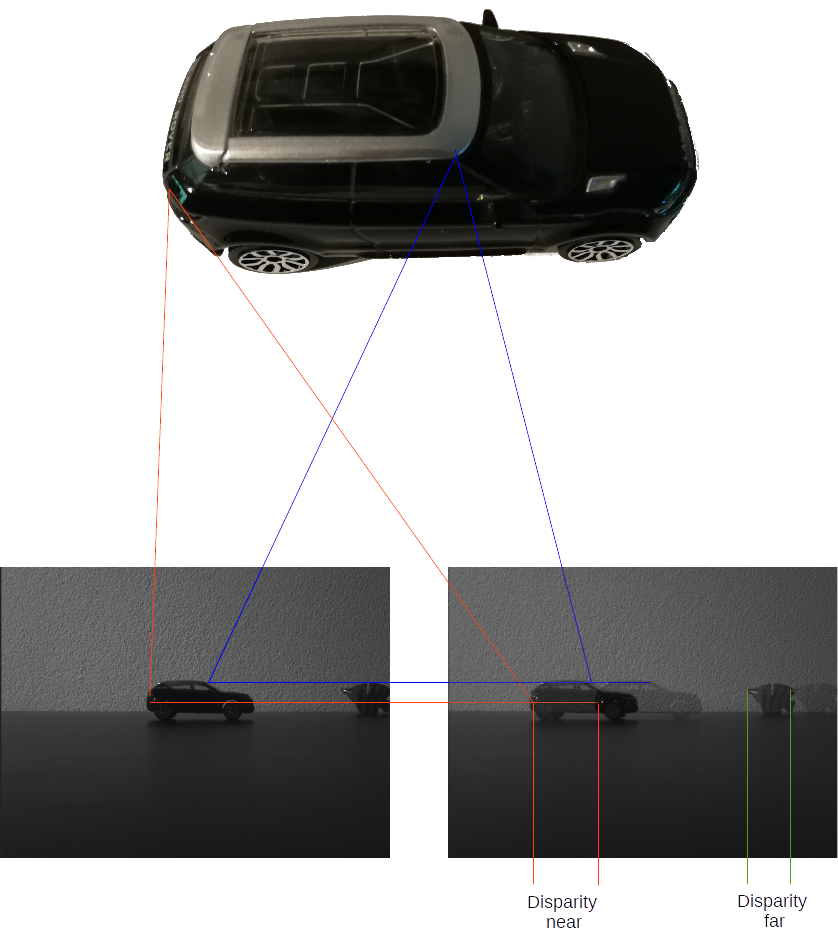
\includegraphics[width=0.9\textwidth]{img/disparity_concept.png}
  \end{center}
  \caption{Disparity with epipolar (horizontal) line, left: left image, right: right image with transparent left image}\label{fig:disparity}
\end{figure}

From the disparity we can calculate the depth (distance from the camera) by using the formula shown in equation \ref{eq:depth_disp}.

\begin{equation}\label{eq:depth_disp}
  Z=\frac{f_m*b*s_{px}}{d}=\frac{f_x*b}{d}
\end{equation}
\begin{align*}
  Z        &: \text{Depth/Distance from camera}\\
  f_x      &: \text{Focal length in pixel}\\
  d        &: \text{Disparity}\\
  b        &: \text{Baseline in meter}\\
  f_m      &: \text{Focal length in meter}\\
  s_{px}  &: \text{Pixel size in meter}
\end{align*}

If we know the pose of the camera we can transform the depth to the global coordinate system. First we need to find calculate the X and Y position in the 3D space with camera as (0,0,0). This is shown in equation \ref{eq:depth_xy}.

\begin{equation}\label{eq:depth_xy}
  \begin{gathered}
    X = \frac{x-c_x}{f_x*Z}\\
    Y = \frac{y-c_y}{f_y*Z}\\
  \end{gathered}
\end{equation}
\begin{align*}
  X,Y,Z    &: \text{Point coordinates with Camera 0,0,0}\\
  f_x,f_y  &: \text{Focal length in pixel}\\
  c_x,c_y  &: \text{Image center (where z axis goes through)}\\
  x,y      &: \text{2D point in image}
\end{align*}

Now we can simply transform the 3D point with camera as reference to the global coordinate system by using the camera pose. This is shown in equation \ref{eq:depth_global}.

\begin{equation}\label{eq:depth_global}
  \begin{pmatrix}
    X'\\
    Y'\\
    Z'
  \end{pmatrix}=
  \begin{pmatrix}
    r_{11} & r_{12} & r_{13}\\
    r_{21} & r_{22} & r_{23}\\
    r_{31} & r_{32} & r_{33}\\
  \end{pmatrix}
  \begin{pmatrix}
    X\\
    Y\\
    Z
  \end{pmatrix}
  +\begin{pmatrix}
    t_x\\
    t_y\\
    t_z
  \end{pmatrix}
\end{equation}
\begin{align*}
  X,Y,Z      &: \text{Point coordinates with Camera 0,0,0}\\
  X',Y',Z'  &: \text{Global point coordinates}\\
  r_{ij}    &: \text{Camera rotation matrix}\\
  t_{x,y,z}  &: \text{Camera location}
\end{align*}



\chapter{Optical Flow}\label{ch:opt_flow}
To speed up the optimization a predefined gradient can be calculated. The method to find such a gradient is related to the Lucas-Kanade optical flow method. Instead of searching a Warp matrix we search a transformation matrix in this scenario. We have two images $I_{k-1}$ and $I_{k}$. We know the pose of image k-1 $T_{k-1}$ . We search the pose $T_k$.\\
While the inverse compositional Lucas Kanade algorithm tries to find the optimal Warp matrix. We try to find the optimal pose.
\section{Lucas Kanade Intuitive}

As mentioned in the previous section Lucas Kanade is an algorithm to estimate the optical flow. In the simplest case it just tells us where a certain pixel was in the image before and where it is now. It does that in a efficient way by using the intensity gradients. This section tries to describe how this works in an intuitive but simplified way while the next section will describe it in a more mathematical way.\\
Let's assume the simplest scenario where we can only move in one direction (left or right). Figure \ref{fig:optical_flow_intuitive} shows this simple scenario. Let's first focus on the case where we have a small movement (a). We first calculate the intensity gradients in the template (first row). Then we calculate the intensity difference (last row) between the current image (second row) and the first image. Now we multiply the gradient times the intensity difference this will give us the direction in which we have to move. Here we assume that moving the current image to left means - and moving it to right +. Now we move in the direction of the gradient and will calculate the intensity difference again. If it increases we moved too much and we have to reduce the step size if it decreases we are fine and we can calculate the new gradient again based on the new intensity difference. After some iterations the intensity change from one iteration to the other should be minimal. We have found the horizontal movement of our image. We already describe the inverse compositional Lucas Kanade algorithm because we calculate the gradients on the template. The ``normal'' Lucas Kanade would calculate the gradients on the current image. This has the disadvantage that we need to calculate the gradients after each iteration and it's therefore less computational efficient.\\
What we can see in \ref{fig:optical_flow_intuitive} (b) that it's impossible to track movements over bigger distances. If the patch we compare does not connect to the area where the new image has moved, we are unable to move in the right direction. As we can see it's even possible that we move in the wrong direction (b). To overcome this problem we can downsample the image as shown in (c). We only downsampled in horizontal direction for visability. In reality the whole image would be downsampled by factor 2,4,8,16, etc. This is called an optical pyramid. As we can see in (c) after we downsampled the image by factor two we have again a valid gradient which points in the right direction. The idea is that we start to optimized in the lowest level if we converge we optimize again one level higher and so on. With this idea it is possible to track flows over higher distances while still being efficient.

\begin{figure}[H]
  \centering
  \subfloat[Lucas Kanade small move]{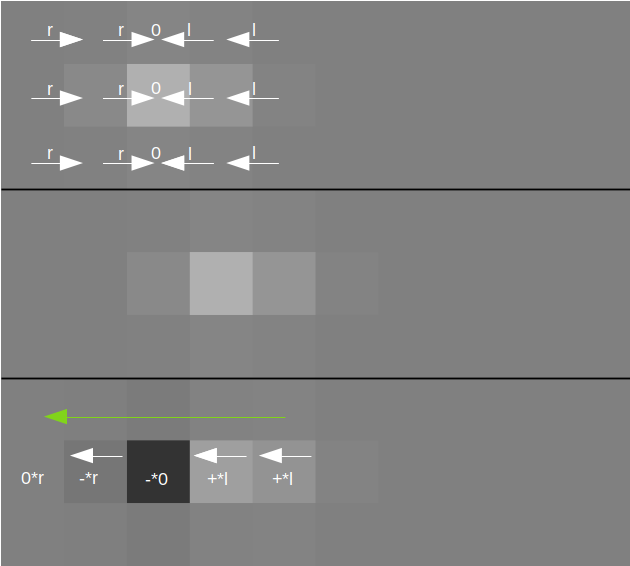
\includegraphics[height=0.2\textheight]{img/optical_flow_intuitive_1.png}}
  \subfloat[Lucas Kanade big move]{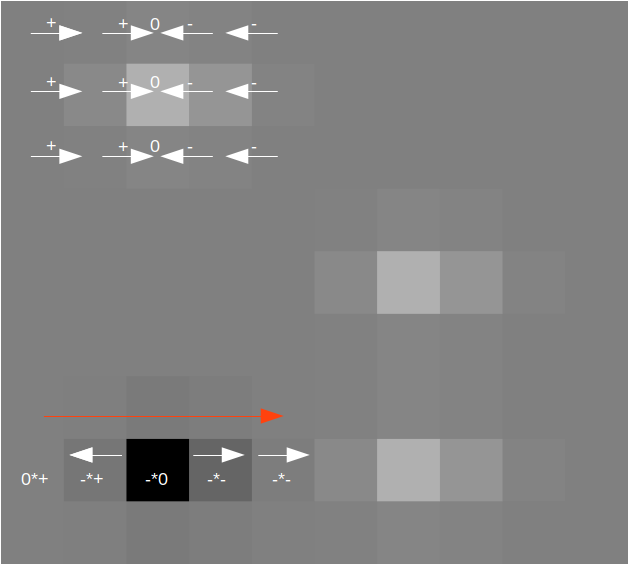
\includegraphics[height=0.2\textheight]{img/optical_flow_intuitive_2.png}}
  \subfloat[Lucas Kanade big move down sampled]{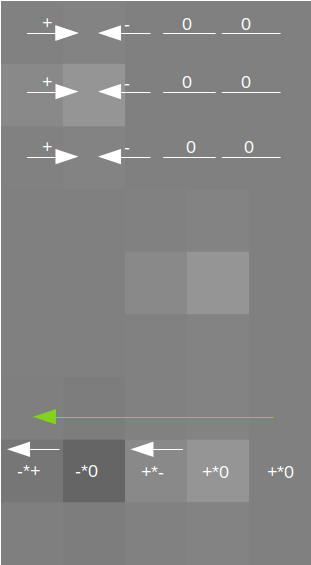
\includegraphics[height=0.2\textheight]{img/optical_flow_intuitive_3.png}}
  \caption{Optical Flow Intuitive}\label{fig:optical_flow_intuitive}
\end{figure}

We can extend the above scenario from a movement in one dimension easily to two dimensions as shown in figure \ref{fig:optical_flow_2d}. We simply calculate the gradient in the vertical direction as well. By doing this we can track movements in x and y direction. We easily see that not all values in the patch help to find the right gradient. Some gradients in the patch point in the wrong direction. However, in total the gradient points in the right direction. By using image pyramids we can reduce the influence of such miss matches.
\begin{figure}[H]
  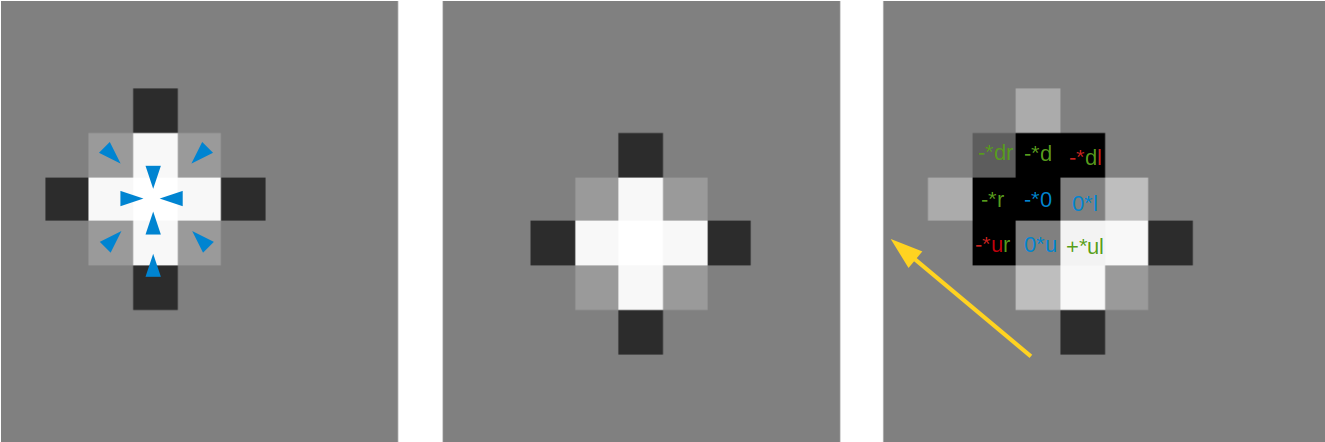
\includegraphics[width=1.0\textwidth]{img/optical_flow_2d.png}
  \caption{Optical Flow Intuitive 2D: +: current-previous intensity > 0, -: current-previous intensity < 0, u: gradient points up, d: gradient points down, l: gradient points left, r: gradient points right, red: wrong direction, green: right direction, blue: no influence, yellow arrow: final gradient}\label{fig:optical_flow_2d}
\end{figure}

We showed that optical flow can track two dimensional movements. However, it doesn't track rotations and shearing. This will introduce dependencies between x and y movements which become non-linear. In the next section we extend the intuitive approach so that we can solve non-linear problems.

\section{Lucas Kanade Mathematical}

In the previous section we showed the basic idea of optical flow. It is oversimplified and can only track movements in x and y direction. In this section we extend this idea so that more complicated movements can be tracked.\\

Instead of linear movements in x and y direction we want to find a warp matrix which describes a affine transformation of a patch from one image to the other (equation \ref{eq:lk_warp}).
\begin{equation}\label{eq:lk_warp}
  p=\begin{pmatrix}
    p_{11} & p_{12} & p_{13} \\
    p_{21} & p_{22} & p_{23}
  \end{pmatrix}
\end{equation}
\begin{align*}
  p        &:  \text{warp matrix}\\
  p_{ij}  &:  \text{parameter of warp matrix}
\end{align*}
This warp matrix describes movements along the x and y axis($p_{11},p_{22}$, a rotation ($p_{13},p_{21}$) and shearing ($p_{13},p_{23}$). The goal of Lucas Kanade is to find this warp matrix. It does that by minimizing the Intensity difference between patch of pixels in a template (reference image) and a patch of pixels with the same size in the current image as shown in equation \ref{eq:lk_problem}. 

\begin{equation}\label{eq:lk_problem}
  \sum_x\sum_y(I_{k}(x',y')-I_{k-1}(x,y))^2
\end{equation}
\begin{align*}
  x,y        &:  \text{Pixel position in template}\\
  x',y'      &:  \text{Pixel position in current image}\\
  I_{k-1}    &:  \text{Template image}\\
  I_{k}      &:  \text{Current image}
\end{align*}

We describe the transformation of a pixel from the reference image to the current image as a matrix multiplication as shown in equation \ref{eq:lk_warped}. Because \ref{eq:lk_problem} is a nonlinear problem we have to solve it with a nonlinear solver (e.g. Gauss-Newton or Gradient Descent). The problem is solved by iteratively changing the warp matrix in the direction of a gradient until the difference of the intensities are minimal:
\begin{equation}\label{eq:lk_warped}
  \begin{gathered}
    \begin{pmatrix}
      x' \\
      y'
    \end{pmatrix}=
    W(x;p+\Delta p)\\
    =>
    \begin{pmatrix}
      p_{11}+\Delta p_{11} & p_{12}+\Delta p_{12} & p_{13}+\Delta p_{13} \\
      p_{21}+\Delta p_{21} & p_{22}+\Delta p_{22} & p_{23}+\Delta p_{23}
    \end{pmatrix}
    \begin{pmatrix}
      x\\
      y\\
      1
    \end{pmatrix}\\
    =>
    \begin{pmatrix}
      x(p_{11}+\Delta p_{11}) + y(p_{12}+\Delta p_{12}) + p_{13}+\Delta p_{13} \\
      x(p_{21}+\Delta p_{21}) + y(p_{22}+\Delta p_{22}) + p_{23}+\Delta p_{23}
    \end{pmatrix}
  \end{gathered}
\end{equation}
\begin{align*}
  W(x;p+\Delta p)  &:  \text{Warp function}\\
  x',y'            &:  \text{Pixel position in current image}\\
  x,y              &:  \text{Pixel position in template}\\
  p_{ij}          &:  \text{parameter of warp matrix}\\
  \Delta p_{ij}    &:  \text{change of $p_{ij}$ per iteration}
\end{align*}

After each iteration we set $p=p_{n-1}+\Delta p$ where p stands for all $p_{ij}$. We can solve this problem by approximating the gradient heuristically. However, this is slow. Therefore, we need a direct computational approach to find the gradient. This is what Lucas Kanade describes. \\
Equation \ref{eq:lk_problem} describes the Lucas Kanade problem which is non linear. It's not possible to find $\Delta p$ algebraicly which would be our gradient. Therefore, we need to linearise the problem by doing a first order Taylor approximation as shown in equation \ref{eq:lk_taylor}. $\nabla I$ corresponds here to the exterior derivative when using the chain rule while $\frac{\sigma W}{\sigma p}$ corresponds to the inner derivative. $\Delta p$ is the factor used for Taylor series (see \cite{taylor_series}).

\begin{equation}\label{eq:lk_taylor}
  \sum_x\sum_y(I_{k}(x_{i-1}',y_{i-1}')+\nabla I_{k}*\frac{\sigma W}{\sigma p}*\Delta p-I_{k-1}(x,y))^2
\end{equation}
\begin{align*}
  x,y        &:  \text{Pixel position in template}\\
  x',y'      &:  \text{Pixel position in current image}\\
  I_{k-1}    &:  \text{Template image}\\
  I_{k}      &:  \text{Current image}\\
  \nabla I  &:  \text{Gradient in image I at position x',y'}
\end{align*}
We want to find $\Delta p$ which is our gradient. To make this work we have to derive equation \ref{eq:lk_taylor}. This gives us:
\begin{equation}
  2*\sum_x\sum_y\begin{bmatrix}\nabla I_{k}*\frac{\sigma W}{\sigma p}\end{bmatrix}^T*\begin{bmatrix}I_{k}(x_{i-1}',y_{i-1}')+\nabla I_{k}*\frac{\sigma W}{\sigma p}*\Delta p-I_{k-1}(x,y)\end{bmatrix}
\end{equation}
We can now find $\Delta p$ by moving it to the left:
\tiny
\begin{equation}\label{eq:lk_dp}
  \Delta p=(\sum_x\sum_y\begin{bmatrix}\nabla I_{k}\frac{\sigma W}{\sigma p}\end{bmatrix}^T\begin{bmatrix}\nabla I_{k}\frac{\sigma W}{\sigma p}\end{bmatrix})^{-1}
  \sum_x\sum_y\begin{bmatrix}\nabla I_{k}\frac{\sigma W}{\sigma p}\end{bmatrix}^T\begin{bmatrix}I_{k-1}(x,y) - I_{k}(x_{i-1}',y_{i-1}'\end{bmatrix}
\end{equation}
\normalsize

To  get $\frac{\sigma W}{\sigma p}$ we take equation \ref{eq:lk_warped} and do a partial derivation for each p which gives us equation \ref{eq:lk_warped_derivative}.
\begin{equation}\label{eq:lk_warped_derivative}
  \frac{\sigma W}{\sigma p}=
  \begin{pmatrix}
    x & y & 1 & 0 & 0 & 0 \\
    0 & 0 & 0 & x & y & 1
  \end{pmatrix}
\end{equation}

All parameters in equation \ref{eq:lk_dp} are known and can be calculated for a given x,y and p. However, the following part of equation \ref{eq:lk_dp} is time consuming to calculate and has to be inverted:
\begin{equation}
  \Delta H=(\sum_x\sum_y\begin{bmatrix}\nabla I_{k}*\frac{\sigma W}{\sigma p}\end{bmatrix}^T*\begin{bmatrix}\nabla I_{k}*\frac{\sigma W}{\sigma p}\end{bmatrix})
\end{equation}
H is called the Hessian matrix. It is the same formulation used by Gauss-Newton optimization. Therefore, we use Gauss-Newton when using $\Delta p$ for the update step \cite{inverse_compositional} during optimization. Unfortunately we need to calculate the Hessian matrix in each iteration. The inverse compositional Lucas Kanade algorithm tries to solve this problem by wrapping the template to the current image instead of the current image to the template.

\section{Inverse compositional Lucas Kanade}

The inverse compositional Lucase Kanade algorithm does more or less the same as the normal Lucas Kanade algorithm but it searches the inverse warp update at each iteration. The problem basically stays the same but we switch the role of the template with the one of the image which first doesn't have any effect:
\begin{equation}\label{eq:iclk_problem}
  \sum_x\sum_y(I_{k-1}(x'',y'')-I_{k}(x',y'))^2
\end{equation}
\begin{align*}
  x'',y''    &:  \text{Warped pixel position in the template}\\
  x',y'      &:  \text{Pixel position in the current image}\\
  I_{k-1}    &:  \text{Template image}\\
  I_{k}      &:  \text{Current image}
\end{align*}

What is different this time is that we warp the template with $\Delta p$ as shown in equation \ref{eq:inv_lk_warp}. 
\begin{equation}\label{eq:inv_lk_warp}
  \begin{gathered}
    \begin{pmatrix}
      x'' \\
      y''
    \end{pmatrix}=
    W(x;\Delta p)\\
    =>\begin{pmatrix}
      1 + \Delta p_{11} & 0 + \Delta p_{12} & 0 + \Delta p_{13} \\
      0 + \Delta p_{21} & 1 + \Delta p_{22} & 0 + \Delta p_{23}
    \end{pmatrix}
    \begin{pmatrix}
      x\\
      y\\
      1
    \end{pmatrix}
  \end{gathered}
\end{equation}
\begin{align*}
  x,y            &:  \text{Original pixel position in template}\\
  x'',y''        &:  \text{Warped pixel position in template}\\
  \Delta p_{ij}  &:  \text{change of $p_{ij}$ per iteration}
\end{align*}

\begin{equation}
  \begin{pmatrix}
    x' \\
    y'
  \end{pmatrix}=
  \begin{pmatrix}
    p_{11} & p_{12} & p_{13} \\
    p_{21} & p_{22} & p_{23}
  \end{pmatrix}*
  \begin{pmatrix}
    x\\
    y\\
    1
  \end{pmatrix}
\end{equation}
\begin{align*}
  x',y'          &:  \text{Pixel position in current image}\\
  x,y            &:  \text{Original pixel position in template}\\
  p_{ij}        &:  \text{parameter of warp matrix}\\
\end{align*}

With this we separate the update step from the warping of the image. The update step is now shown in equation \ref{eq:iclk_update}. Note that this time the update step is not additive as for normal Lucas Kanade. This is where the word compositional comes from. We can argue that this time the new warp depends on the old warps rotation because the template is always free from rotation. This can be expressed with a matrix multiplication also shown in equation \ref{eq:iclk_update}.
\begin{equation}\label{eq:iclk_update}
  \begin{gathered}
    W(x;p)=W(W(x;\Delta p)^{-1}; p)\\
    =>
    \begin{pmatrix}
    p_{11} & p_{12} & p_{13} \\
    p_{21} & p_{22} & p_{23}
    \end{pmatrix}
    \begin{pmatrix}
      \Delta p_{11} & \Delta p_{12} & \Delta p_{13} \\
      \Delta p_{21} & \Delta p_{22} & \Delta p_{23}
    \end{pmatrix}
    \begin{pmatrix}
      x\\
      y\\
      1
    \end{pmatrix}
  \end{gathered}
\end{equation}

From equation \ref{eq:iclk_problem} we need to do the first order Taylor approximation as we did for the normal Lucas Kanade algorithm. This is shown in equation \ref{eq:iclk_taylor}.
\begin{equation}\label{eq:iclk_taylor}
  \sum_x\sum_y(I_{k-1}(x,y)+\nabla I_{k-1}*\frac{\sigma W}{\sigma p}*\Delta p-I_{k}(x',y'))^2
\end{equation}
\begin{align*}
  x,y        &:  \text{Original pixel position in template}\\
  x',y'      &:  \text{Pixel position in current image}\\
  I_{k-1}    &:  \text{Template image}\\
  I_{k}      &:  \text{Current image}\\
  \nabla I  &:  \text{Gradient in image I at position x',y'}
\end{align*}

We derive equation \ref{eq:iclk_taylor} and set it to zero so that we can minimize the problem (equation \ref{eq:iclk_derivative}).
\begin{equation}\label{eq:iclk_derivative}
  2\sum_x\sum_y\begin{bmatrix}\nabla I_{k-1}\frac{\sigma W}{\sigma p}\end{bmatrix}^T\begin{bmatrix}I_{k}(x_{i-1}',y_{i-1}')+\nabla I_{k-1}\frac{\sigma W}{\sigma p}\Delta p-I_{k-1}(x,y)\end{bmatrix}
\end{equation}

This allows us to find the gradient $\Delta p$ (equation \ref{eq:iclk_dp}) for the non linear optimization.
\tiny
\begin{equation}\label{eq:iclk_dp}
  \Delta p=(\sum_x\sum_y\begin{bmatrix}\nabla I_{k-1}\frac{\sigma W}{\sigma p}\end{bmatrix}^T\begin{bmatrix}\nabla I_{k-1}\frac{\sigma W}{\sigma p}\end{bmatrix})^{-1}
  \sum_x\sum_y\begin{bmatrix}\nabla I_{k-1}\frac{\sigma W}{\sigma p}\end{bmatrix}^T\begin{bmatrix}I_{k}(x_{i-1}',y_{i-1}') - I_{k-1}(x,y)\end{bmatrix}
\end{equation}
\normalsize

Compared to the normal Lucas-Kanade algorithm the Hessian Matrix H is now constant for all iterations and we don't have to do the expensive calculation at every iteration:
\begin{equation}
  \Delta H=\sum_x\sum_y\begin{bmatrix}\nabla I_{k-1}*\frac{\sigma W}{\sigma p}\end{bmatrix}^T*\begin{bmatrix}\nabla I_{k-1}*\frac{\sigma W}{\sigma p}\end{bmatrix}
\end{equation}

Because we only have to calculate the Hessian matrix once, the inverse computational Lucas Kanade is more efficient then the Lucas Kanade algorithm.\\
In this chapter we saw how we calculate the optical flow by using a warp matrix. As we will later see this is used by SVO in the pose refinement step. In the next section we describe how optical flow can be used to find a 3D pose instead of a warp matrix.

\section{Pose Estimation}\label{sec:pose_estimation}
For a first estimate of the pose we use some kind of optical flow algorithm. However, we directly try to find the 3D pose instead of the warp matrix. Also we don't try to find a warp matrix for each individual patch but for all patches in the image. We start again with the idea of minimizing the intensity differences over a patch of pixels shown in equation \ref{eq:pe_problem}.
\begin{equation}\label{eq:pe_problem}
  \sum_x\sum_y(I_{k-1}(x'',y'')-I_{k}(x',y'))^2
\end{equation}
\begin{align*}
  x'',y''    &:  \text{Warped pixel position in the template}\\
  x',y'      &:  \text{Pixel position in the current image}\\
  I_{k-1}        &:  \text{Template image}\\
  I_{k}          &:  \text{Current image}
\end{align*}

This time we use 3D points instead of pixel positions. Therefore, we use a projection matrix instead of a warp matrix. The projection matrix $p$ is shown in equation \ref{eq:pe_warped}. 

\begin{equation}\label{eq:pe_warped}
  \begin{split}
  \begin{pmatrix}
    u \\
    v \\
    s
  \end{pmatrix}=
  \begin{pmatrix}
    f_x & 0 & c_x \\
    0 & f_y & c_y \\
    0 & 0 & 1
  \end{pmatrix}*
  \begin{pmatrix}
    r_{11} & r_{12} & r_{13} & t_{1} \\
    r_{21} & r_{22} & r_{23} & t_{2} \\
    r_{31} & r_{32} & r_{33} & t_{3}
  \end{pmatrix}*
  \begin{pmatrix}
    X\\
    Y\\
    Z\\
    1
  \end{pmatrix}\\
  =>\begin{pmatrix}
    p_{11} & p_{12} & p_{13} & p_{14} \\
    p_{21} & p_{22} & p_{23} & p_{24} \\
    p_{31} & p_{32} & p_{33} & p_{34}
  \end{pmatrix}*
  \begin{pmatrix}
    X\\
    Y\\
    Z\\
    1
  \end{pmatrix}
\end{split}
\end{equation}
\begin{align*}
  u,v,s      &:  \text{Pixel position scaled with s}\\
  X,Y,Z      &:  \text{3D Pixel position}\\
  p_{ij}    &:  \text{Projection matrix}\\
\end{align*}

We would need to find 12 gradients if we use the formulation in equation \ref{eq:pe_projection} for the inverse compositional Lucas Kanade. However, the rotational factors $r_{nm}$ in equation \ref{eq:pe_warped} depend on each other. We could express the whole matrix based on 6 unknowns which are 3 times rotation and 3 times translation. Unfortunately it is easy to see that this formulation gets rather complex and it's nearly impossible to find a Jacobian for such a matrix.\\

\begin{equation}\label{eq:pe_projection}
  \begin{gathered}
    \begin{pmatrix}
      x' \\
      y' 
    \end{pmatrix}=
    \begin{pmatrix}
      \frac{u}{s} \\
      \frac{v}{s} 
    \end{pmatrix}=
    \begin{pmatrix}
      \frac{p_{11}*X + p_{12}*Y + p_{13}*Z + p_{14}}{p_{31}*X + p_{32}*Y + p_{33}*Z + p_{34}}  \\
      \frac{p_{21}*X + p_{22}*Y + p_{23}*Z + p_{24}}{p_{31}*X + p_{32}*Y + p_{33}*Z + p_{34}}
    \end{pmatrix}\\
    \begin{pmatrix}
      x'' \\
      y'' 
    \end{pmatrix}=W(x,y,z;\Delta p)\\
    =>\begin{pmatrix}
      \frac{u'}{s'} \\
      \frac{v'}{s'} 
    \end{pmatrix}=
    \begin{pmatrix}
      \frac{\Delta p_{11}*X + \Delta p_{12}*Y + \Delta p_{13}*Z + \Delta p_{14}}{\Delta p_{31}*X + \Delta p_{32}*Y + \Delta p_{33}*Z + \Delta p_{34}}  \\
      \frac{\Delta p_{21}*X + \Delta p_{22}*Y + \Delta p_{23}*Z + \Delta p_{24}}{\Delta p_{31}*X + \Delta p_{32}*Y + \Delta p_{33}*Z + \Delta p_{34}}
    \end{pmatrix}\\
  \end{gathered}
\end{equation}
\begin{align*}
  u,v,s      &:  \text{Pixel position scaled with s}\\
  X,Y,Z      &:  \text{3D Pixel position}\\
  p_{ij}    &:  \text{Projection matrix}\\
\end{align*}

We reformulate the problem by using Lie algebra. The idea is to transform the angles and translations into another space where we can find a Jacobian. The optimization is done in this space. The result of the optimization is transformed from Lie algebra back to angles and translations which we can use to update the pose for the next iteration. The problem we need to solve stays the same as in equation \ref{eq:pe_problem}. However we need to find $x''$ and $y''$ differently. We use the following formulation:
\begin{equation}\label{eq:pe_lie}
  \begin{gathered}
    \begin{pmatrix}
      x''\\
      y''
    \end{pmatrix}
    =h(e^{\xi}*p)\\
    \xi=\begin{pmatrix}
      v_x\\
      v_y\\
      v_z\\
      \omega_x\\
      \omega_y\\
      \omega_z
    \end{pmatrix}
  \end{gathered}
\end{equation}
\begin{align*}
  h      &:  \text{Mapping function from u,v,s to x,y}\\
  e      &:  \text{Exponential map}\\
  \xi    &:  \text{Pose change between reference frame and current frame as vector in SE(3)}\\
  p      &:  \text{point in 3D cloud}
\end{align*}

$\xi$ in \ref{eq:pe_lie} is the change in angle and position in Lie algebra. We can transfer from Lie algebra back to SE(3) which is our ``normal'' space by using the exponential map $e$. The exponential map is the pendant to the Euler function for matrices. In our case it has the closed form solution shown in \ref{eq:pe_closed_form} \cite{rvc}.

\begin{equation}\label{eq:pe_closed_form}
  \begin{gathered}
    \omega_{skew}=\begin{pmatrix}
      0 && -\omega_z && \omega_y \\
      \omega_z && 0 && -\omega_x \\
      -\omega_y && \omega_x && 0
    \end{pmatrix}\\
    \begin{pmatrix}
      \Delta t_x\\
      \Delta t_y\\
      \Delta t_z
    \end{pmatrix}=
    I+(1-cos(1))w_{skew}+(1-sin(1))*w_{skew}^2*\begin{pmatrix}
      v_x\\
      v_y\\
      v_z
    \end{pmatrix}\\
    \begin{pmatrix}
      \Delta r_x\\
      \Delta r_y\\
      \Delta r_z
    \end{pmatrix}=
    \begin{pmatrix}
      \omega_x\\
      \omega_y\\
      \omega_z
    \end{pmatrix}
  \end{gathered}
\end{equation}

We use $\Delta t_x,\Delta t_y,\Delta t_z,\Delta r_x,\Delta r_y,\Delta r_z$ as our gradient for optimizing the pose. To get $\xi$ we again do the first order Taylor approximation as shown in equation \ref{eq:pe_taylor}).
\begin{equation}\label{eq:pe_taylor}
  \sum_x\sum_y(I_{k-1}(x,y)+\nabla I_{k-1}*\frac{\sigma h(e^{\xi}*p)}{\sigma \xi}*\xi-I_{k}(x',y'))^2
\end{equation}
\begin{align*}
  h      			&:  \text{Mapping function from u,v,s to x,y}\\
  x,y        	&: \text{Original pixel position in template}\\
  x',y'      	&: \text{Pixel position in current image}\\
  I_{k-1}    	&: \text{Template image}\\
  I_{k}      	&: \text{Current image}\\
  \nabla I  	&: \text{Gradient in image I at position x',y'}\\
  \xi        	&: \text{Twist formulated in Lie algebra}\\
  p          	&: \text{point in 3D space}  
\end{align*}

We again derive equation \ref{eq:pe_taylor} from $\xi$ and set it to zero as shown in equation \ref{eq:pe_derivative}. This finally allows us to find $\xi$.

\begin{equation}\label{eq:pe_derivative}
  2\sum_x\sum_y\begin{bmatrix}\nabla I_{k-1}\frac{\sigma h(e^{\xi}p)}{\sigma \xi}\end{bmatrix}^T\begin{bmatrix}I_{k}(x_{i-1}',y_{i-1}')+\nabla I_{k-1}\frac{\sigma h(e^{\xi} p)}{\sigma \xi}\xi-I_{k-1}(x,y)\end{bmatrix}
\end{equation}

We want to find $\xi$ which leads us to equation \ref{eq:pe_xi}.

\tiny
\begin{equation}\label{eq:pe_xi}
  \xi=(\sum_x\sum_y\begin{bmatrix}\nabla I_{k-1}\frac{\sigma h(e^{\xi}p)}{\sigma \xi}\end{bmatrix}^T\begin{bmatrix}\nabla I_{k-1}\frac{\sigma h(e^{\xi}p)}{\sigma \xi}\end{bmatrix})^{-1}
  \sum_x\sum_y\begin{bmatrix}\nabla I_{k-1}\frac{\sigma h(e^{\xi}p)}{\sigma \xi}\end{bmatrix}^T\begin{bmatrix}I_{k}(x_{i-1}',y_{i-1}') - I_{k-1}(x,y)\end{bmatrix}
\end{equation}
\normalsize

We now only have to find a solution for $\frac{\sigma h(e^{\xi}p)}{\sigma \xi}$ to be able to caclulate $\xi$. This Jacobian matrix is shown in equation \ref{eq:se3_jacobian} \cite{se3_explain}.

\begin{equation}\label{eq:se3_jacobian}
  \frac{h(e^{\xi}p)}{\delta \xi}=
  \begin{pmatrix}
    f_x & f_y
  \end{pmatrix}
  \begin{pmatrix}
    \frac{1}{z} & 0 & -\frac{x}{z^2} & -\frac{x*y}{z^2} & 1 + \frac{x^2}{z^2} & -\frac{y}{z} \\
    0 & \frac{1}{z}  & -\frac{y}{z^2} & -1 - \frac{y^2}{z^2} & \frac{x*y}{z^2} &  \frac{x}{z}
  \end{pmatrix}
\end{equation}
\begin{align*}
  f_x,f_y  &:  \text{Focal length}\\
  x,y,z    &:  \text{3D point position}\\
\end{align*}

Given the Jacobian, all 3D points we can now calculate the gradient for a given pose and then iteratively optimize the pose pased on the gradient. Becasue we again use the Inverse Compositional Lucas Kanade approach, the Hessian only needs to be calculated once per optimization step and not for each iteration.

\chapter{Pose Refinement}\label{ch:pose_refinement}

Pose refinement is used to decrease the drift over time and to increase the accuracy of the pose estimation. In a first step we use optical flow to locate keypoints from the keyframe in the current image. Then we try to minimize the reprojection error shown in equation \ref{eq:refinement_reprojection}.
\begin{equation}\label{eq:refinement_reprojection}
  \begin{gathered}
    minimize(\sum_n ((x'-x)^2+(y'-y)^2))\\
    =>minimize(\sum_n ((L'-L)^T(L'-L))
  \end{gathered}
\end{equation}
\begin{align*}
  x',y'   &: \text{Keypoint position found by optical flow}\\
  x,y     &: \text{Keypoint projection from 3D cloud with camera pose see \ref{eq:camera_model}}\\
  n       &: \text{count of keypoints}\\
  L,L'    &: \text{x,y and x',y' as vector}
\end{align*}

We could do that with e.g. heuristic gradient descent. However, this would be again computationally inefficient because for each iteration we would have to do up to 7 calculations. Therefore, we try to use a similar approach as we use for optical flow. We try to find the gradient mathematically. Let take again the equation \ref{eq:pe_projection}. We don't use the exact same definition but instead use the formulation shown in equation \ref{eq:refinement_projection}. Again we don't want to use this formulation directly. Some parameters depend on each other (rotational) and we can't find a Jacobian for this formulation.

\begin{equation}\label{eq:refinement_projection}
  \begin{gathered}
    \begin{pmatrix}
      x \\
      y 
    \end{pmatrix}=
    \begin{pmatrix}
      \frac{u}{s} \\
      \frac{v}{s} 
    \end{pmatrix}=
    \begin{pmatrix}
      \frac{(p_{11} + \Delta p_{11})*X + (p_{12} + \Delta p_{12})*Y + (p_{13} + \Delta p_{13})*Z + (p_{14} + \Delta p_{14})}{(p_{31}+\Delta p_{31})*X + (p_{32} + \Delta p_{32})*Y + (p_{33} + \Delta p_{33})*Z + (p_{34} + \Delta p_{34})}  \\
      \frac{(p_{21} + \Delta p_{21})*X + (p_{22} + \Delta p_{22})*Y + (p_{23} + \Delta p_{23})*Z + (p_{24} + \Delta p_{24})}{(p_{31}+\Delta p_{31})*X + (p_{32} + \Delta p_{32})*Y + (p_{33} + \Delta p_{33})*Z + (p_{34} + \Delta p_{34})}
    \end{pmatrix}
  \end{gathered}
\end{equation}
\begin{align*}
  u,v,s           &:  \text{Pixel position scaled with s}\\
  X,Y,Z           &:  \text{3D Pixel position}\\
  p_{ij}          &:  \text{Projection matrix}\\
  \Delta p_{ij}   &:  \text{Projection matrix change per iteration}\\
\end{align*}

We now formulate the problem again with the help of Lie algebra shown in equation \ref{eq:refinement_lie}.
\begin{equation}\label{eq:refinement_lie}
  \begin{gathered}
    \begin{pmatrix}
      x\\
      y
    \end{pmatrix}
    =h(e^{\xi}*p)\\
    \xi=\begin{pmatrix}
      v_x\\
      v_y\\
      v_z\\
      \omega_x\\
      \omega_y\\
      \omega_z
    \end{pmatrix}
  \end{gathered}
\end{equation}
\begin{align*}
  P     &: \text{Current projection matrix}\\
  e     &: \text{Exponential map}\\
  \xi   &: \text{Pose change between reference frame and current frame as vector in SE(3)}\\
  p     &: \text{3D point in camera local coordinates}\\
  h     &: \text{u,v,s to x,y}
\end{align*}

If we formulate the problem of equation \ref{eq:refinement_problem} with the knowledge of equation \ref{eq:refinement_lie} we end up in equation \ref{eq:refinement_solve}.

\begin{equation}\label{eq:refinement_solve}
  \begin{gathered}
    \sum_n ((L'-L)^T(L'-L))\\
    =>\sum_n (L'-h(e^{\xi}*p))^2
  \end{gathered}
\end{equation}

We do a Taylor approximation of the inner part as shown in equation \ref{eq:refinement_taylor}.
\begin{equation}\label{eq:refinement_taylor}
  (L'-h(p)+\frac{h(e^{\xi}*p)}{\xi}(\xi))^2
\end{equation}

Now we derive the Taylor approximation to be able to minimize it. This is shown in equation \ref{eq:refinement_derived}. Keep in mind that the gradient points towards maxima. Therefore, we would optimize in direction of the negative gradient.
\begin{equation}\label{eq:refinement_derived}
  \begin{gathered}
    (\frac{h(e^{\xi}*p)}{\xi})^T2*(L'-h(p)+\frac{h(e^{\xi}*p)}{\xi}(\xi))=0\\
    (\frac{h(e^{\xi}*p)}{\xi})^T(L'-h(p))+\frac{h(e^{\xi}*p)}{\xi}\frac{h(e^{\xi}*p)}{\xi}\xi=0\\
    (\frac{h(e^{\xi}*p)}{\xi})^T(\frac{h(e^{\xi}*p)}{\xi})^{-1}(\frac{h(e^{\xi}*p)}{\xi})^T(h(p)-L')=\xi
  \end{gathered}
\end{equation}

We can reuse the same definition for the Jacobian as we did for pose estimation in equation \ref{eq:se3_jacobian}. The only difference is that this time we use the repojection error instead of the intensity gradient to calculate the gradient.

\chapter{Implementation}\label{ch:implementation}

In this chapter we discuss the implementation that was written during this thesis. It should give a ruff overview of the code base. The whole project is GNU Makefile based. Table \ref{tab:envvars} shows the environment variables be used to control the make process.
\begin{table}[H]
  \centering
  \begin{tabular}{|l|l|}
    Variable & Description\\
    \hline
    OPENCV\_INC\_DIR & Include directory for OpenCV (opencv2/..)\\
    OPENCV\_LIB\_DIR & Where to find the opencv libraries if not in standard path\\
    QT\_INC\_DIR & Where to find the QT include files if not in standard path\\
    QMAKE & Which qmake should be used\\
    CXX & Which compiler should be use\\
    CXXFLAGS & Additional compiler flags (e.g. -O0/-O3)\\
    LDFLAGS & Additional linker flags (e.g.  additional library paths)
  \end{tabular}
\caption{Environment variables for GNU Make}
\label{tab:envvars}
\end{table}

The git repository is organized as follows:
\begin{table}[H]
  \centering
  \begin{tabular}{|l|l|}
    Directory & Description\\
    \hline
    doc & Documentation (current document)\\
    src  & The source code\\
    src/app & The source code for the test application\\
    src/ar-app & The source code for the demo augmented reality app\\
    src/lib & The source code for the library\\
    src/python & The source code for the python wrapper and python demo\\
    src/qt-viewer & The source code for the Qt 3D Viewer\\
    test & Some test and helper scripts that are irrelevant
  \end{tabular}
\caption{Repository organization}
\label{tab:organization}
\end{table}


\section{Library}

The stereo SVO Library (libstereosvo) is written as shared library. It can be used in other project by dynamically linking against it.

\begin{figure}[H]
  \centering
  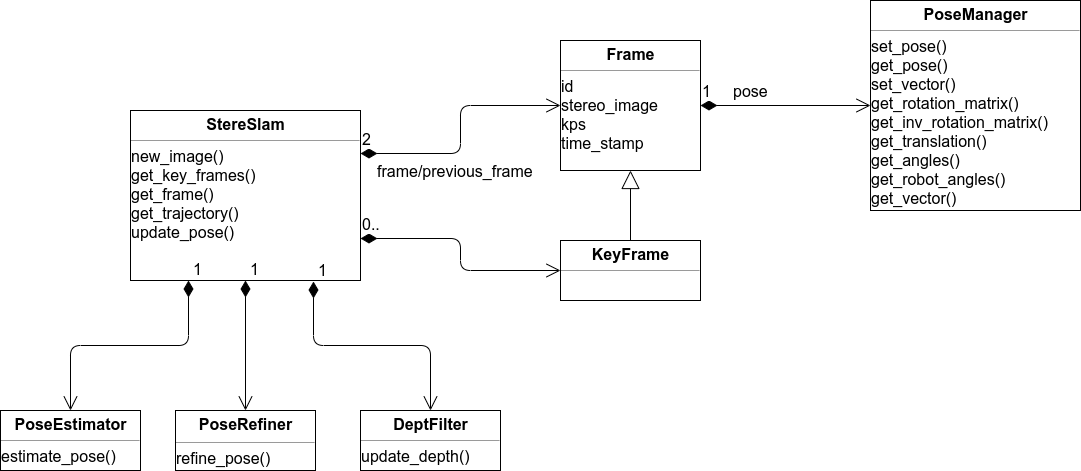
\includegraphics[width=1.0\textwidth]{img/class_diagram.png}
  \caption{Class diagram for the Stereo SVO Library}\label{fig:class_diagram}
\end{figure}

Figure \ref{fig:class_diagram} shows the most important classes of the library. There are a lot of other files and data types available. However, they support the main classes in doing their work. An application must create an objection based on StereoSlam. When creating the object we need to specify the camera parameters (see attached documentation). After that we can already feed new images by calling it's method new\_image. The getter function can be used to optain the current frame (with pose information), all keyframes (including keypoints), the trajectory or to update the pose. Updating the pose can be used to feed data from an IMU. Currently this is not tested very well. However, it is possible to feed gyro data which helps to improve the stability of the tracker.

\subsection{Stereo SLAM}

The Stereo SLAM class implements the basic algorithm described in \ref{ch:svo} and shown in \ref{fig:svo_slam}. Figure \ref{fig:flow_stereo_slam} shows a slightly changed flow chart to align better with the naming in the implementation. It calls the depth calculator if new keyframes are needed, estimates the pose and updates the point cloud. However, the work is delegated to its sub objects. It also provides an interface to receive information about the current state (see figure \ref{fig:class_diagram}. The interfaces are described in more detail in the separate source code documentation.

\begin{figure}[H]
  \centering
  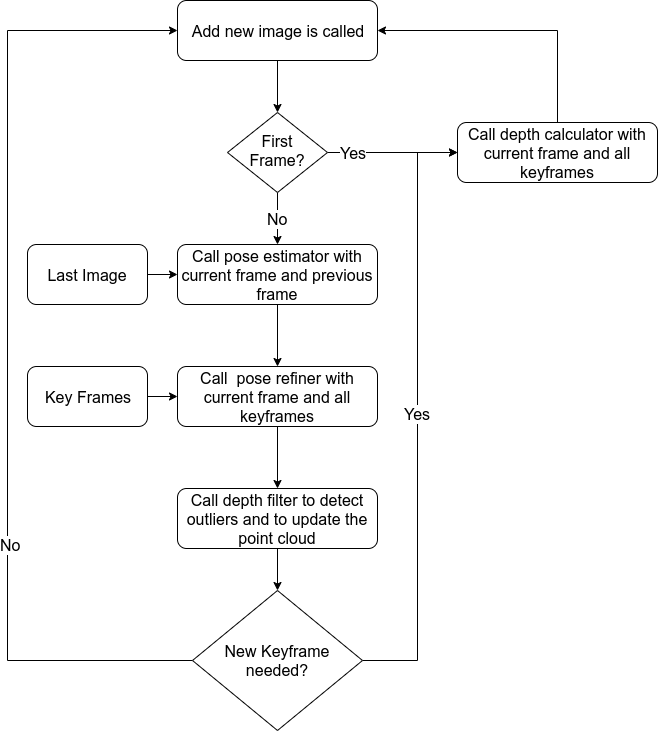
\includegraphics[scale=0.3]{img/flow_stereo_slam.png}
  \caption{Stereo SLAM Flow}\label{fig:flow_stereo_slam}
\end{figure}


\subsection{Depth Calculator}

The depth calculator divides the image into grids and searches for new keypoints, merges keypoints from previous keyframes and estimates the depth. It is only used when a new keyframe is required. Figure \ref{fig:flow_depth_calculator} shows the flow diagram of the depth calculation.

\begin{figure}[H]
  \centering
  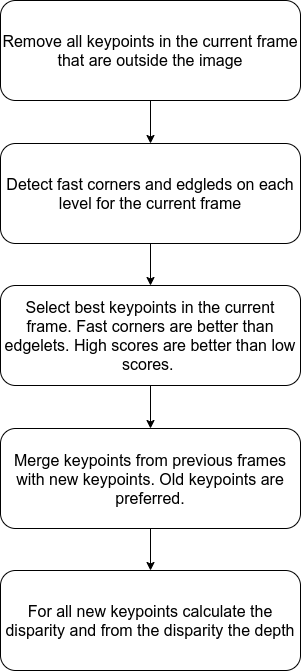
\includegraphics[scale=0.3]{img/flow_depth_calculator.png}
  \caption{Depth Calculator Flow}\label{fig:flow_depth_calculator}
\end{figure}

\subsection{Pose Estimator}

The pose estimator does a first estimate of the pose based on the previous image. It does that by using sparse image alignment described in section \ref{sec:sia}. Figure \ref{fig:flow_pose_estimator} shows the flow diagram for the pose estimator.

\begin{figure}[H]
  \centering
  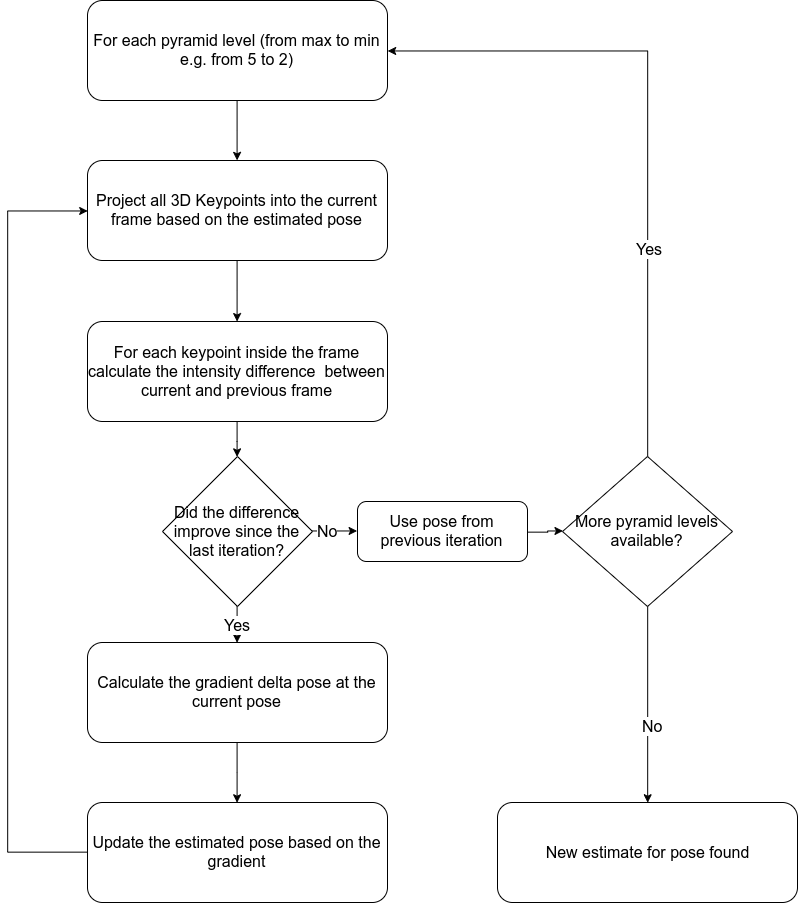
\includegraphics[scale=0.3]{img/flow_pose_estimator.png}
  \caption{Pose Estimator Flow}\label{fig:flow_pose_estimator}
\end{figure}

\subsection{Pose Refiner}

The pose refiner updates the pose by taking the keyframes into account where a keypoint has first been seen. This reduces the drift and makes the pose estimation more stable. It uses the algorithm described in chapter \ref{ch:pose_refinement}. Figure \ref{fig:flow_pose_refiner} shows the flow diagram of the pose refiner.

\begin{figure}[H]
  \centering
  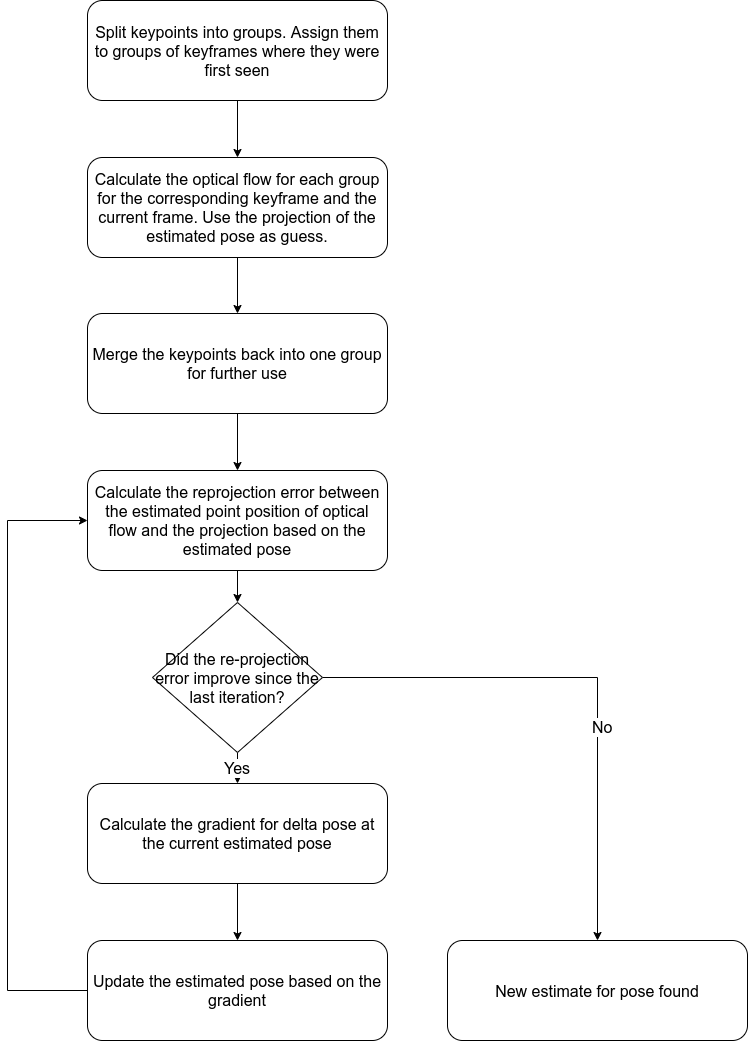
\includegraphics[scale=0.3]{img/flow_pose_refiner.png}
  \caption{Pose Refiner Flow}\label{fig:flow_pose_refiner}
\end{figure}

\subsection{Depth Filter}

The depth filter removes outlier and updates the 3D point position of keypoints. It is completely different from what the original implementation does. The reason is that they work with seeds which we don't require because we use stereo cameras. We don't have seeds but we can improve the 3D points if we have bigger camera movements than the camera baseline is. Figure \ref{fig:flow_depth_filter} shows two flows. The first flow a describes the outlier detection while the second flow b describes the 3D point update.

\begin{figure}[H]
  \centering
  \subfloat[Outlier detecction]{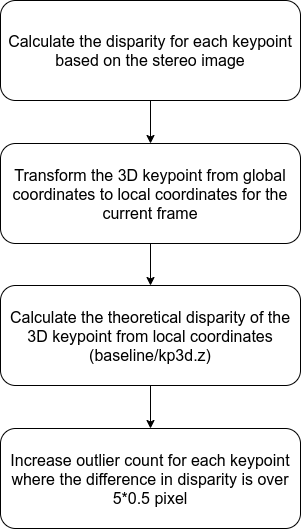
\includegraphics[scale=0.3]{img/flow_depth_filter_outlier.png}}
  \qquad
  \subfloat[3D Point Update]{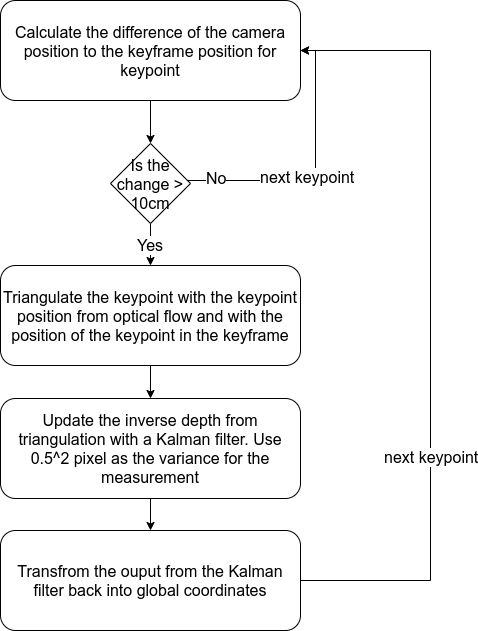
\includegraphics[scale=0.3]{img/flow_depth_filter_update.png}}
  \caption{Depth Filter Flow}\label{fig:flow_depth_filter}
\end{figure}

\section{Test application}

\begin{figure}[H]
  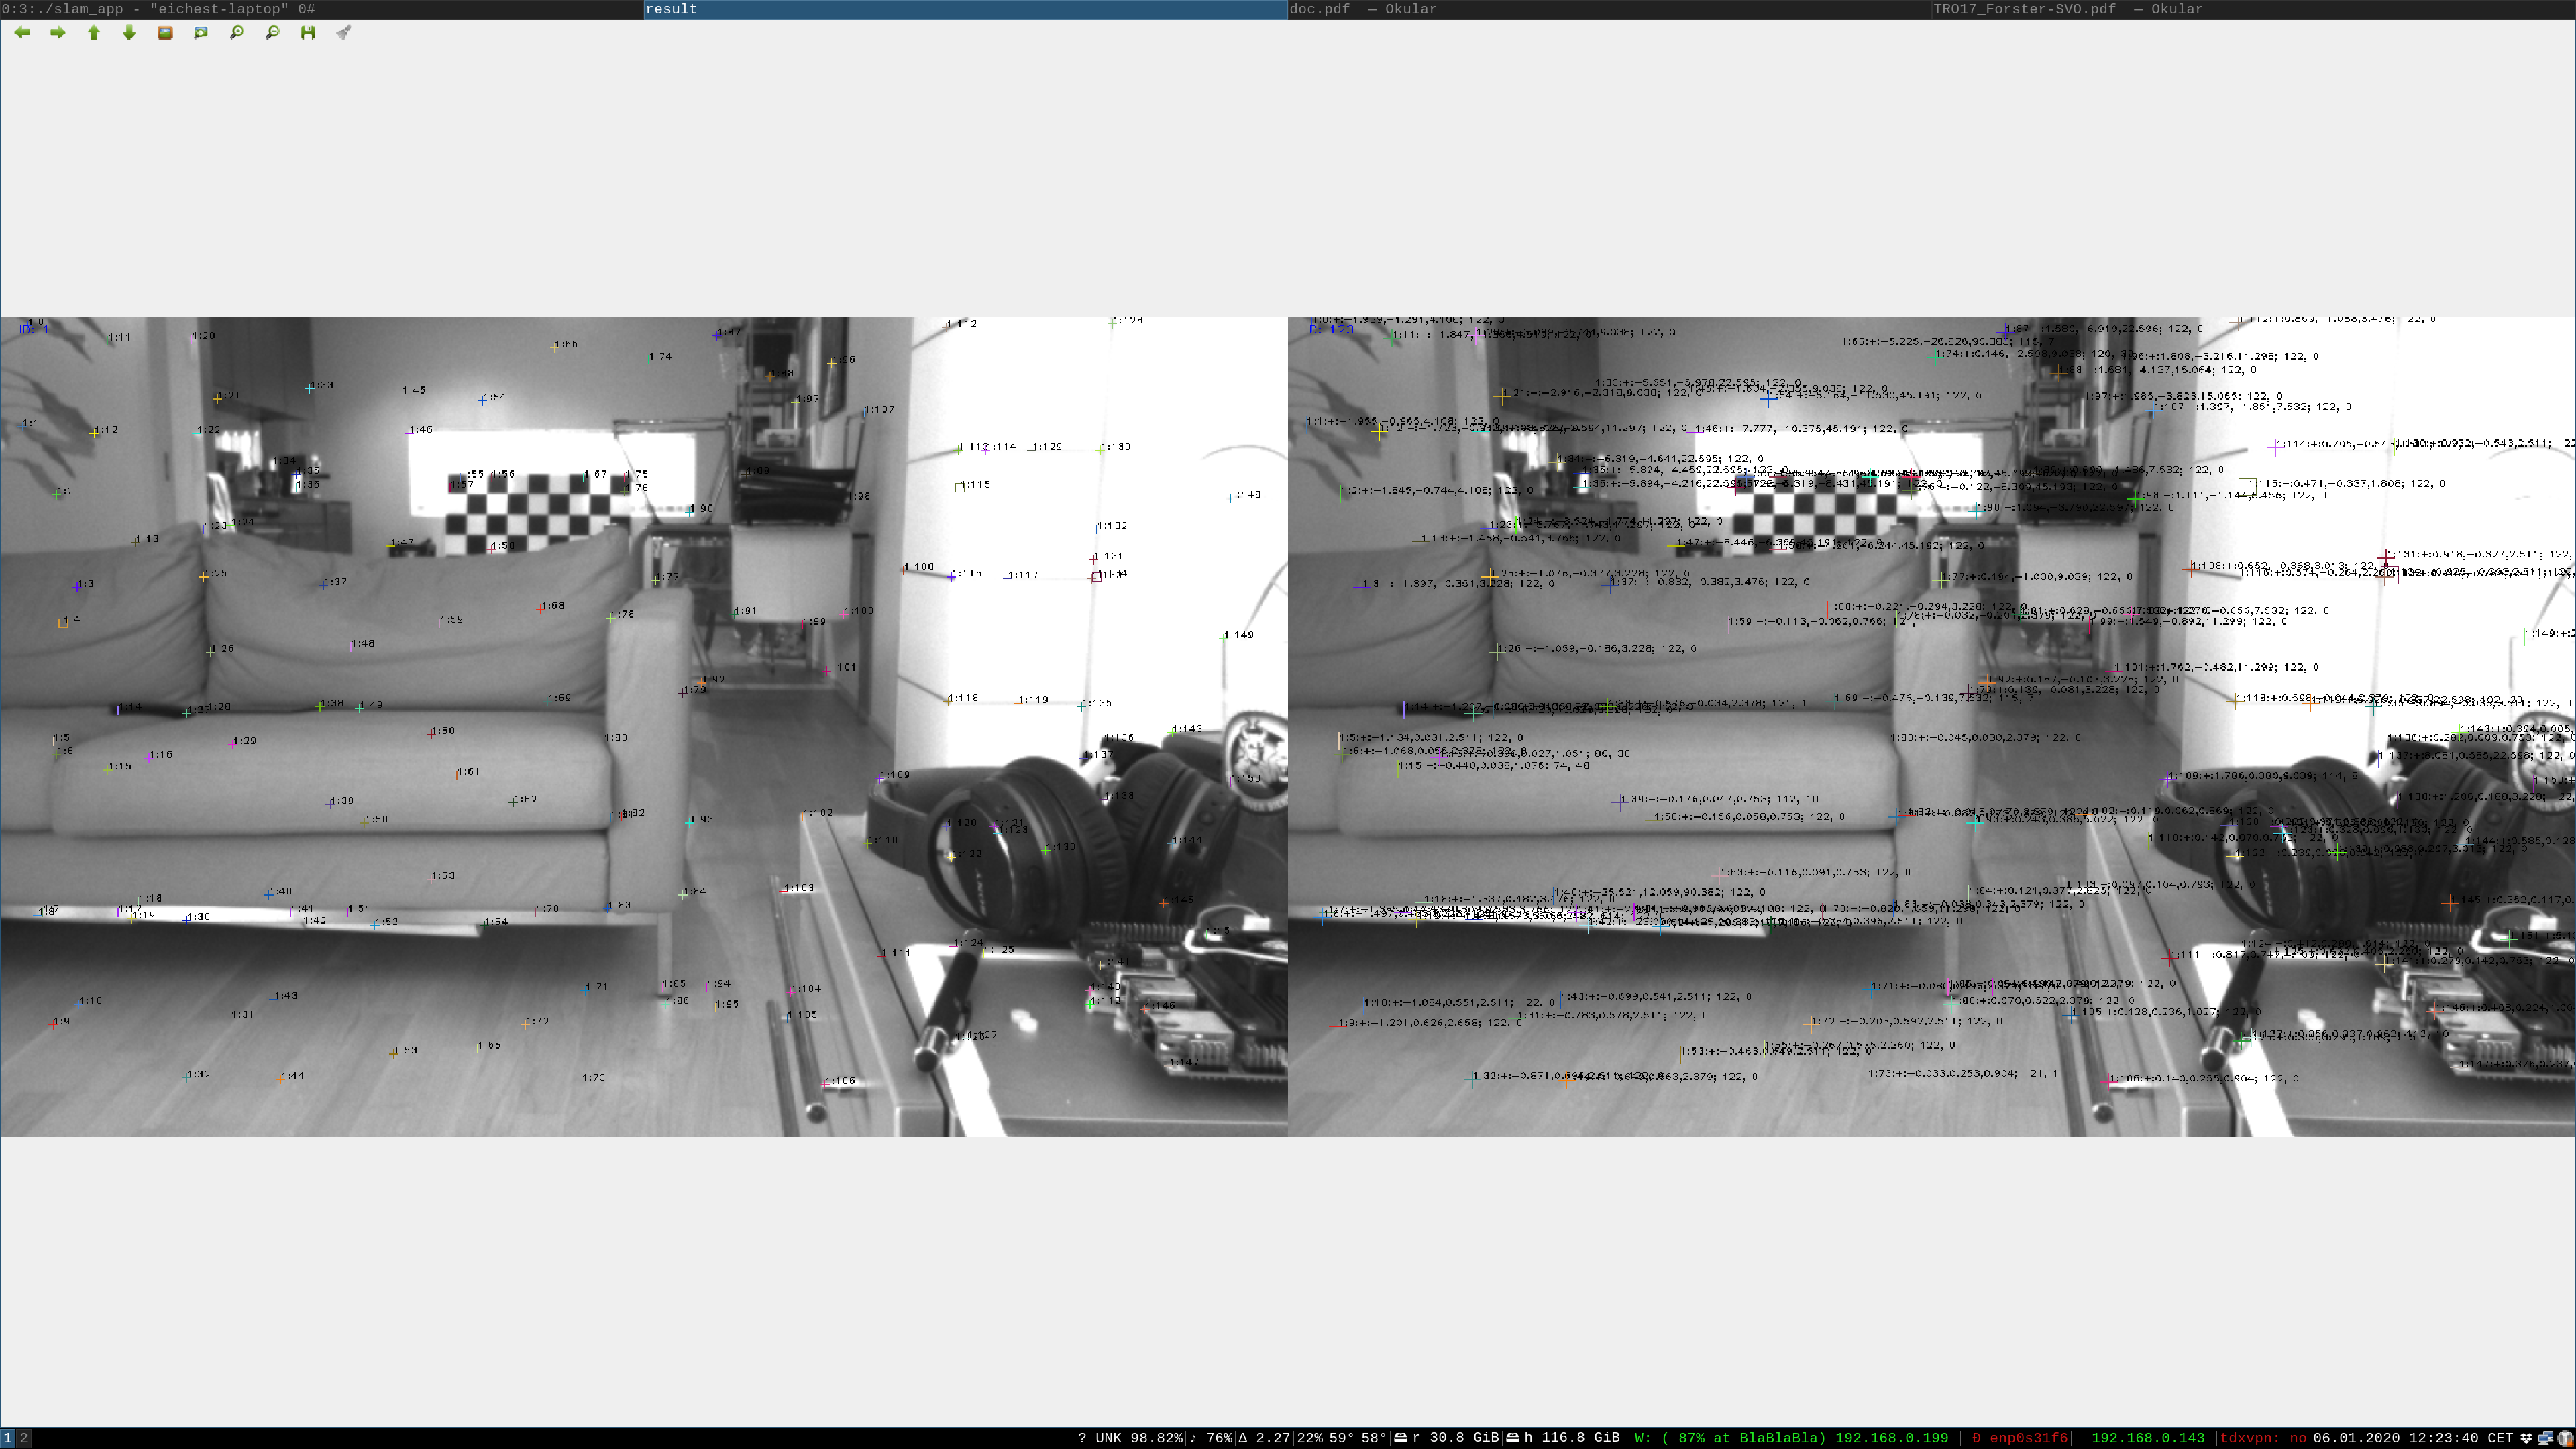
\includegraphics[width=0.9\textwidth]{img/test_app.png}
  \caption{Image from the Test Application}\label{fig:test_app}
\end{figure}

The test application can be used to test the algorithm and to debug it. It allows to use different input sources like video, EuRoC and camera. It also offers a WebSocket interface which allows the Qt Viewer to catch information about the current state of the application. Information that can be received are current camera pose, all keyframe poses, keypoints and trajectory. Figure \ref{fig:test_app} shows an example output of the application. The left side shows the last keyframe with all keypoints that were visible there and the right image show the actual frame. In the keyframe it shows the following numbering a:b. A is the keyframe id where the frame was first seen and b is the index of the keypoint in the keyframe where it was first seen. In the current frame it shows the following information a:b:+/-:x,y,z;inliers,outliers. A and b are again the keypoint ids + means the keypoint is currently used (- would mean it wont be used) then follows the x,y,z position and the last two numbers say how many times the point was counted as inlier or as outlier. The numbers are small but it's possible to zoom in to make them bigger. This numbers are interesting when debugging the application. By pressing a key other than q we can freeze the processing to analyse the current state. By pressing q we can stop the application.\\
Additionally to the above output the test application offers a Websocket \cite{websocket} backend. Through this backend it is possible for the Qt Viewer to read out 3D data like current pose, keyframes and trajectory. The Websocket idea is shown in figure \ref{fig:websocket}.

\begin{figure}[H]
  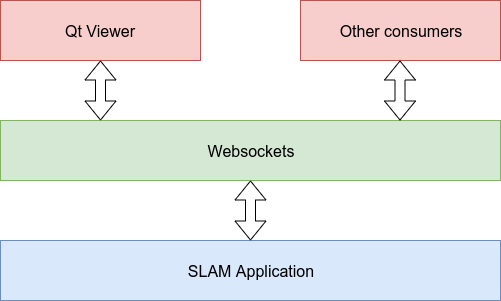
\includegraphics[width=0.9\textwidth]{img/websocket.png}
  \caption{Websocket Connection}\label{fig:websocket}
\end{figure}

It is possible to access via Websocket URLs. Table \ref{tab:websocketapi} shows the implemented commands and URLs. For the trajectory it will send x1,y1,z1,rx1,ry1,rz1,x2,y2,z2,... The test application will open a Websocket port on port 8001.

\begin{table}[H]
  \centering
  \begin{tabular}{|l|l|l|}
    URL & Command & Response \\
    \hline
    keypoints & get & \makecell[l]{\{\\"colors":[\{"b":139,"g":69,"r":103\},\dots],\\"keypoints":[\{"x":-4.8,"y":-0.9,"z":6.1\},\dots],\\pose":\{"rx":0.4,"ry":0.1,"rz":-0.9,"x":-1.8,"y":0.2,"z":0.1\}\\\}}\\
    \hline
    pose & get & \makecell[l]{\{"pose":\{"rx":-9.1,"ry":0.0,"rz":-0.0,"x":-1.2,"y":0.0,"z":-2.0\}\}}\\
    \hline
    trajectory & get & \makecell[l]{\{"trajectory":[0,0,0,0,0,0,0.1,0.1,0.1,0.1,0.1,0.1,0.1,\dots]\}}\\
  \end{tabular}
  \caption{Websocket commands}
  \label{tab:websocketapi}
\end{table}

\section{Qt Viewer}
\begin{figure}[H]
  \centering
  \subfloat[Viewer with reduced keyframes]{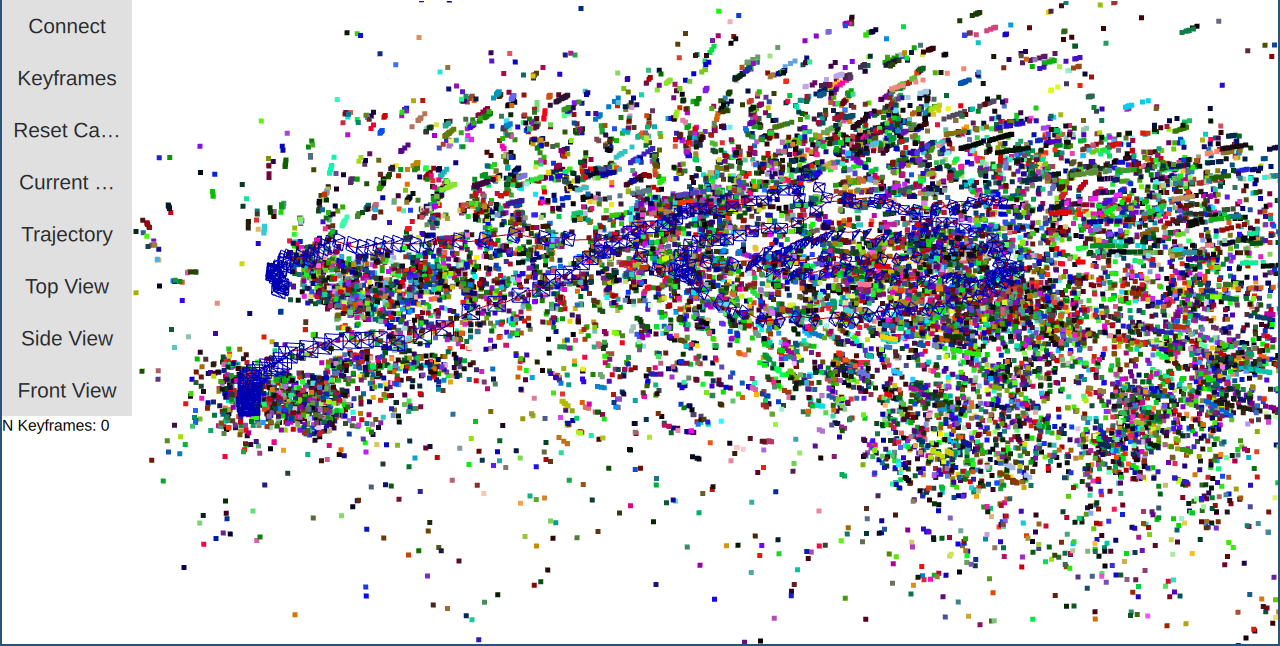
\includegraphics[width=0.45\textwidth]{img/qt_viewer1.png}}
  \qquad
  \subfloat[Viewer with all keyframes]{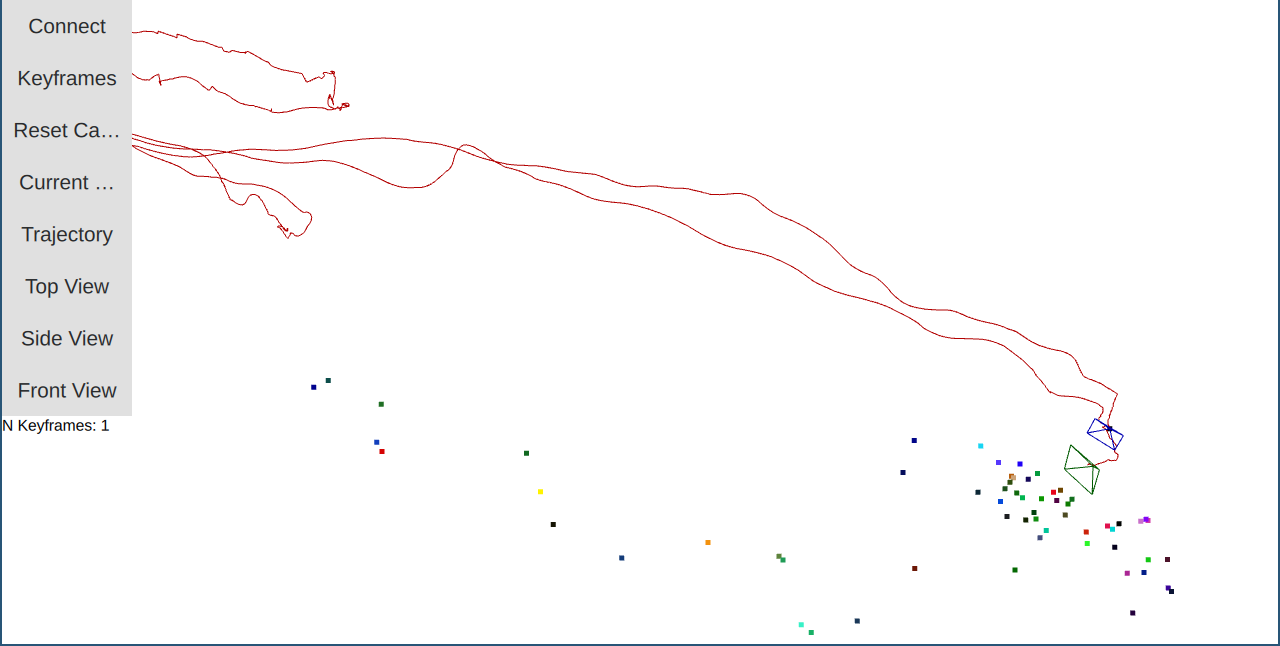
\includegraphics[width=0.45\textwidth]{img/qt_viewer2.png}}
  \caption{Qt Viewer}\label{fig:qt_viewer}
\end{figure}

We can use the Qt Viewer shown in figure \ref{fig:qt_viewer} to display 3D information calculated by the Test Application. We can navigate with the mouse to move trough the 3D room. The data is not received automatically. We need to click connect, get pose, etc. to trigger an action. This allows us to keep a snapshot of a scene to analyse the current state. All points have the same color as in the test application. Keyframes are shown as blue rectangles, the current frame pose is shown in green. The trajectory is shown as red line. When pressing the connect button it will automatically connect to localhost on port 8001, which is where the Test Application is listening on.

\section{Demo application}
\begin{figure}[H]
  \centering
  \subfloat[Demo application first view]{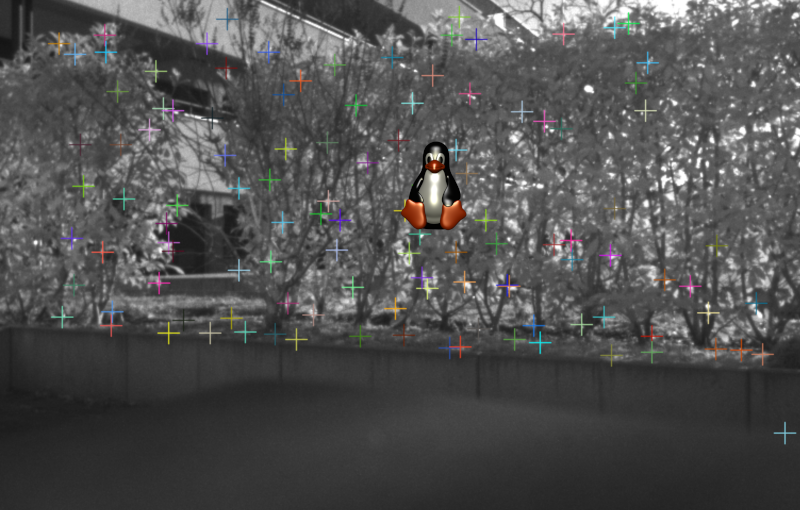
\includegraphics[width=0.45\textwidth]{img/demo_app1.png}}
  \qquad
  \subfloat[Demo application different view]{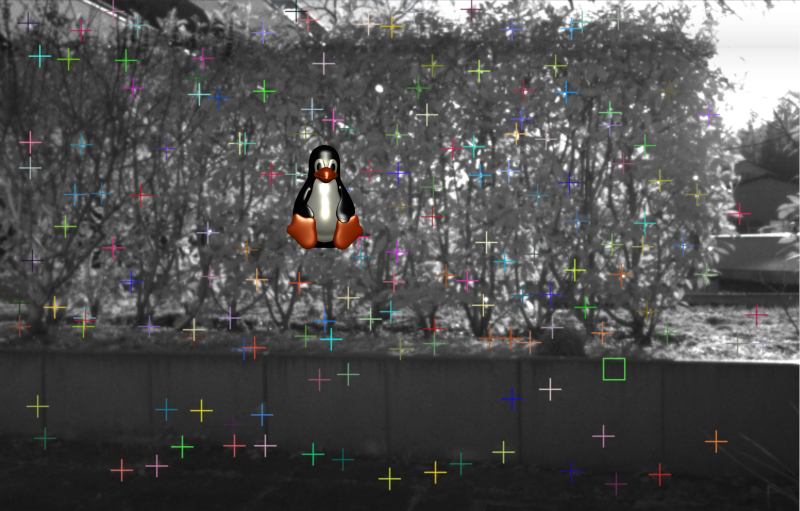
\includegraphics[width=0.45\textwidth]{img/demo_app2.png}}
  \caption{Demo Application}\label{fig:demo_application}
\end{figure}

The demo application shown in figure \ref{fig:demo_application} is a simple augmented reality application that demonstrates one usecase. If we move the camera the Tux should stay at the same place. It is possible to disable the painting of the keypoints by not providing the -p option when starting the application. Only the econ camera is supported as input.

\section{Additional tools}

There are a few other tools available which will not be documented in more detail because they are in bad shape or not intended for further use.

\subsection{Python wrapper}
There is a Python wrapper under src/python which uses Cython to generate bindings. It allows us to use libstereoslam from within Python. A demo application is provided as main.py. It provides a similar feature set as the Test Application.

\subsection{Scripts}
There are several scripts under test which can be used to record videos from the econ camera in the right format. To print the results for the next section, etc.

\chapter{Results}\label{ch:results}

For testing the algorithm with a reference implementation we use a synthetic scene generated by Blender. The advantage of having synthetic scenes is that we can test some well defined movements where we exactly know the trajectory. We compare our implementation with SVO edgelet \cite{svo_edgled} as well as the original SVO implementation \cite{svo}. This is based on the reference SVO implementation. However, it is using newer versions of OpenCV, libegien, etc. They added edgelets tracking which is missing in the original SVO sources and they added a GUI to observe the tracking. However, it's much slower than the original implementation on the other side it seems to be more robust than the original implementation. Unfortunately the reference implementation are quite prone to changes in z and angle changes. Therefore, a simplified scene was generate to have at least some reference. All measurements were done on an Intel i7-8550U processor a version without OpenMP was used (see \ref{ch:implementation}).

\section{Classroom}
\begin{figure}[H]
  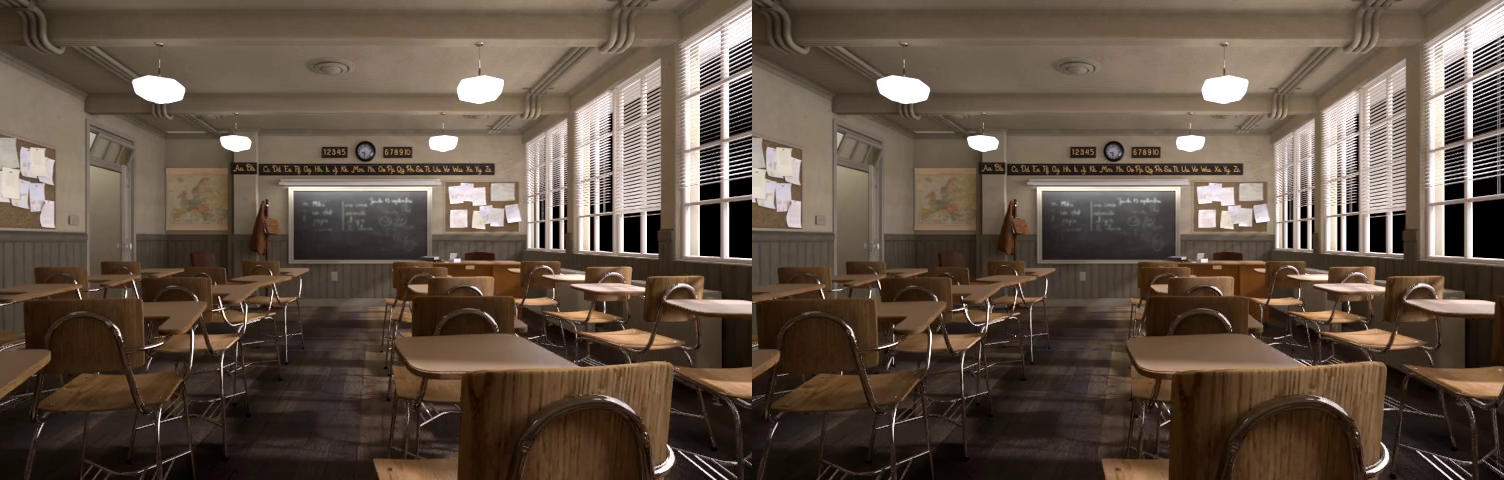
\includegraphics[width=1.0\textwidth]{img/blender_classroom_scene.png}
  \caption{Blender classroom scene}\label{fig:blender_classroom_scene}
\end{figure}

For the first test we use the Blender Classroom Scene \cite{blender}. A snapshot from this scene is shown in figure \ref{fig:blender_classroom_scene}. An image for the left and right camera was rendered to have a valid stereo image input. We change the position and angles in this scene as shown in figure \ref{fig:blender_classroom_simple_traj}.

\begin{figure}[H]
  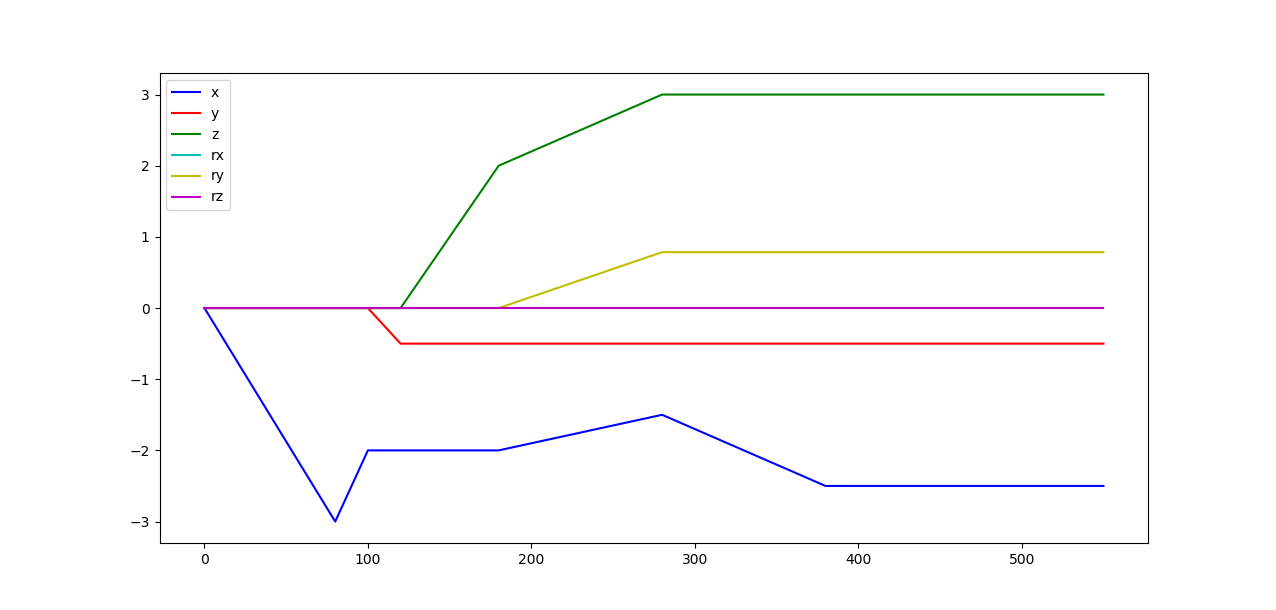
\includegraphics[width=1.0\textwidth]{img/blender_classroom_simple_traj.png}
  \caption{Blender classroom trajectory}\label{fig:blender_classroom_simple_traj}
\end{figure}

Figure \ref{fig:blender_classroom_simple_diff} shows the trajectory difference measured by our implementation, the SVO edgeled reference and the orignal SVO implementation. Both reference implementations are scaled to make a comparison possible. Table \ref{tab:maximas} show the maximum error, table \ref{tab:average} the average error and table \ref{tab:fps} shows the average frames per seconds when doing the measurement.

\begin{table}[H]
  \centering
  \begin{tabular}{|c|c|c|c|c|c|c|}
    impl & err x & err y & err z & err rx & err ry & err rz\\
    \hline
    Our SVO & 0.031 & 0.013 & 0.073 & 0.205 & 0.610 & 0.285\\
    Edgled SVO & 0.344 & 0.099 & 0.273 & 0.989 & 12.941 & 1.430\\
    Original SVO & 0.300 & 0.120 & 0.488 & 1.169 & 6.123 & 1.390\\
    ORB SLAM& 0.023 & 0.015 & 0.023 & 0.222 & 0.302 & 0.204
  \end{tabular}
  \caption{Maximum errors in meter (x,y,z) and Degrees (rx,ry,rz)}
  \label{tab:maximas}
\end{table}

\begin{table}[H]
  \centering
  \begin{tabular}{|c|c|c|c|c|c|c|}
  impl & err x & err y & err z & err rx & err ry & err rz\\
  \hline
  Our SVO & 0.008 & 0.005 & 0.032 & 0.110 & 0.390 & 0.107\\
  Edgled SVO & 0.158 & 0.050 & 0.093 & 0.477 & 5.349 & 0.344\\
  Original SVO & 0.060 & 0.058 & 0.202 & 0.396 & 3.132 & 0.557\\
  ORB SLAM & 0.006 & 0.004 & 0.011 & 0.074 & 0.084 & 0.123
\end{tabular}

\caption{Average errors in meter (x,y,z) and Degrees (rx,ry,rz)}
\label{tab:average}
\end{table}

\begin{table}[H]
  \centering
  \begin{tabular}{|c|c|}
  impl & FPS\\
  \hline
  Our SVO & 52.38\\
  Edgled SVO & 0.93\\
  Original SVO & 115.81\\
  ORB SLAM & 17.38
\end{tabular}
\caption{Frame rate}
\label{tab:fps}
\end{table}

As we see in the results all implementations have a hard time to track the ry angle and the z movment. Both is expected because the with a change in ry we can often correct small movments along the x axis. When moving along the z axis we are not able to refine the 3D point positions because we don't get any change along the x or y axis. This makes it impossible for monocular systems to insert new keypoints.

\begin{figure}[H]
  \subfloat[Our implementation]{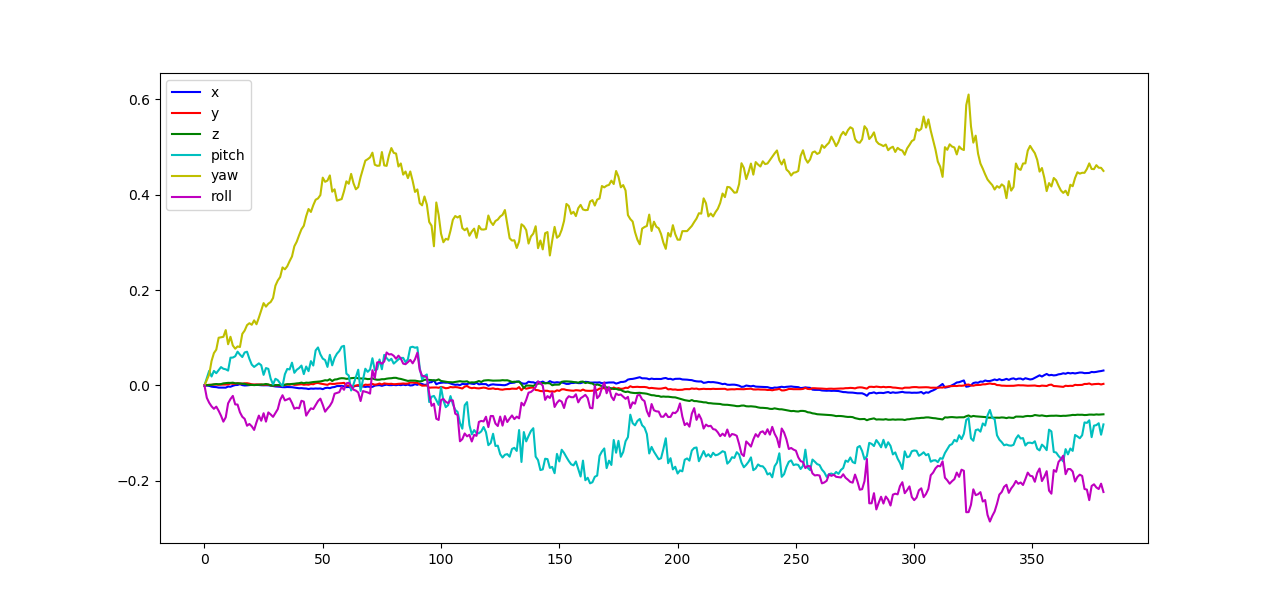
\includegraphics[width=0.5\textwidth]{img/blender_classroom_simple_our_diff.png}}
  \subfloat[SVO Edgled implementation]{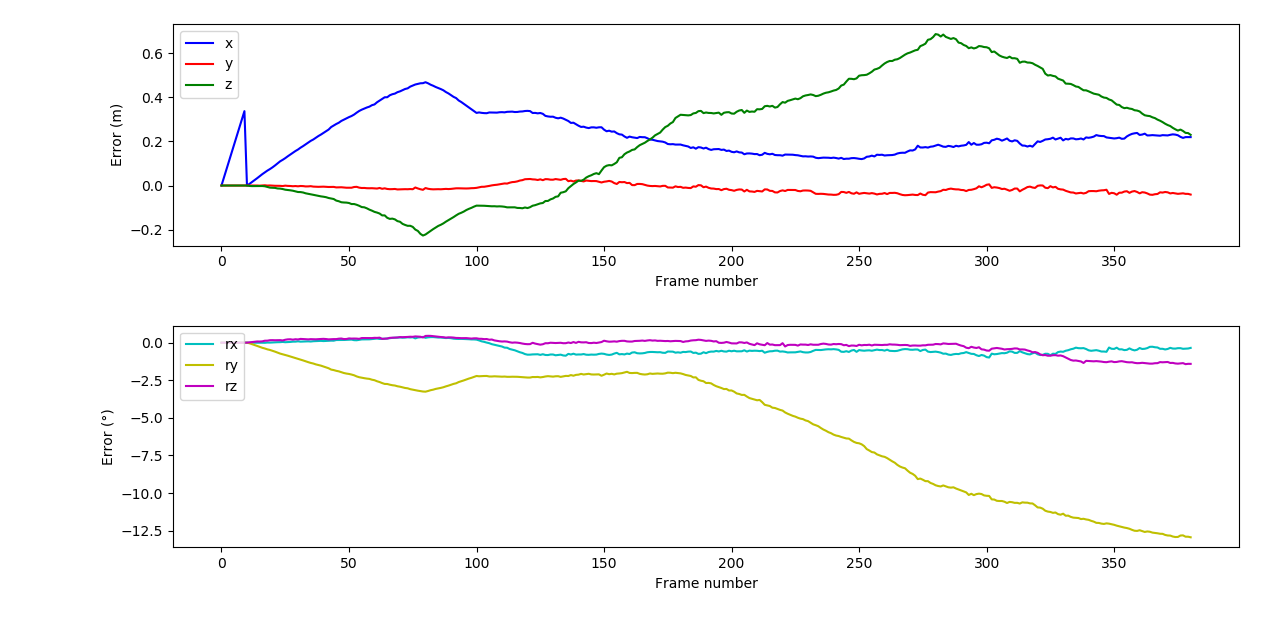
\includegraphics[width=0.5\textwidth]{img/blender_classroom_simple_ref_diff.png}}\\
  \subfloat[SVO Original implementation]{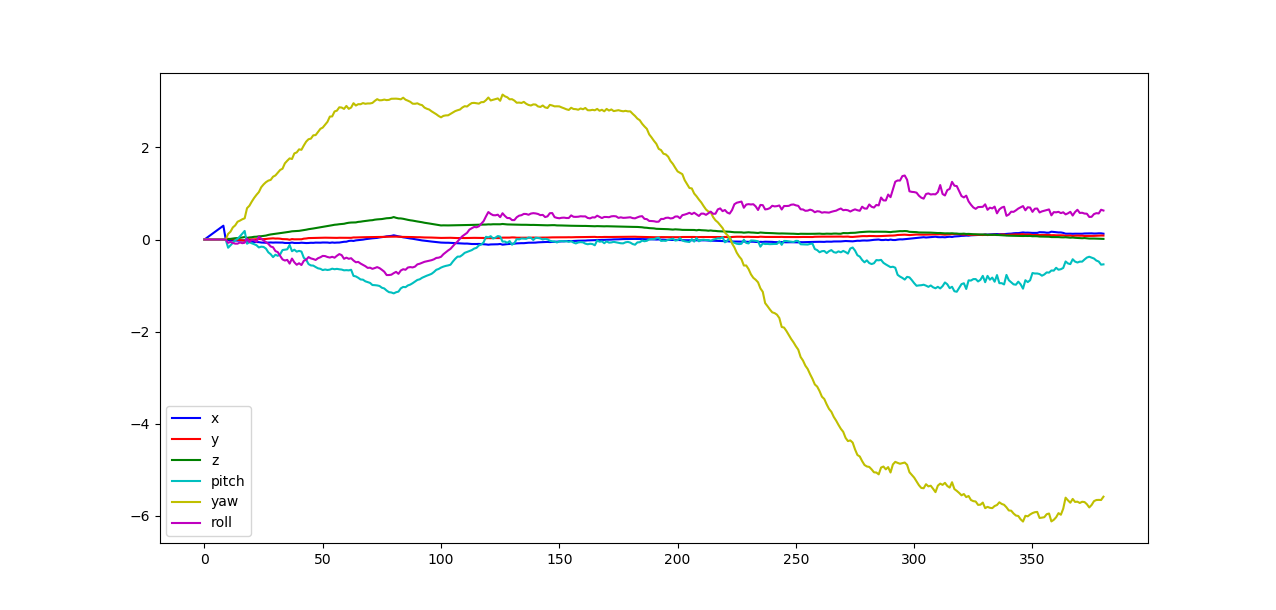
\includegraphics[width=0.5\textwidth]{img/blender_classroom_simple_orig_diff.png}}
  \subfloat[ORB SLAM]{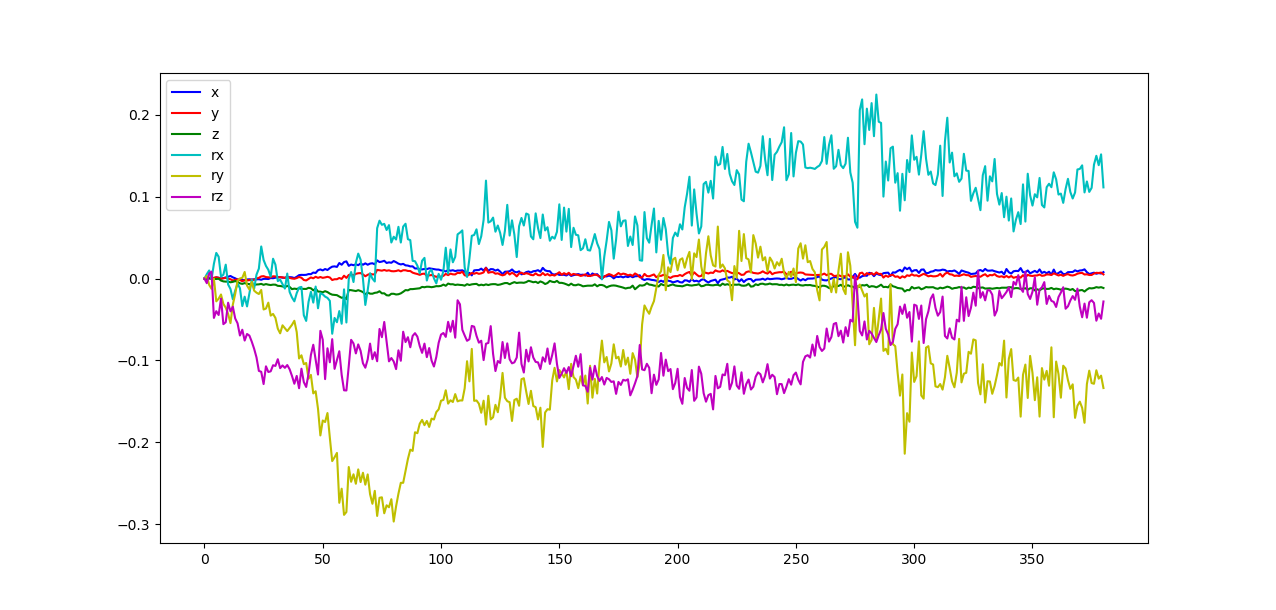
\includegraphics[width=0.5\textwidth]{img/blender_classroom_simple_orb_diff.png}}
  \caption{Blender classroom Scene errors. Distances in meter, angels in Degree.}\label{fig:blender_classroom_simple_diff}
\end{figure}

\section{Barcelona}

\begin{figure}[H]
  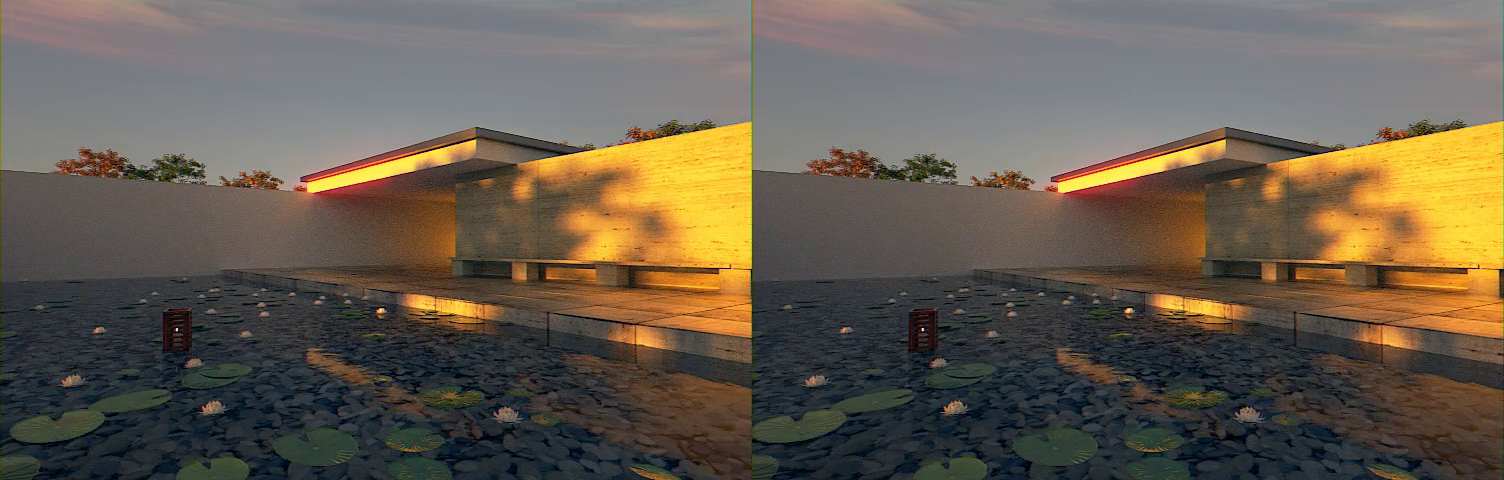
\includegraphics[width=1.0\textwidth]{img/blender_barcelona_scene.png}
  \caption{Blender Barcelona scene}\label{fig:blender_barcelona_scene}
\end{figure}

For the second test we use an outdoor synthetic scene called Barcelona \cite{blender}. Here we only compare ORB SLAM with our SVO implementation because the monocular SLAMs are unable to track such complicated movements. Figure \ref{fig:blender_barcelona_traj} shows the trajectory. The challenges for the tracker are long z movement and big changes in angle.

\begin{figure}[H]
  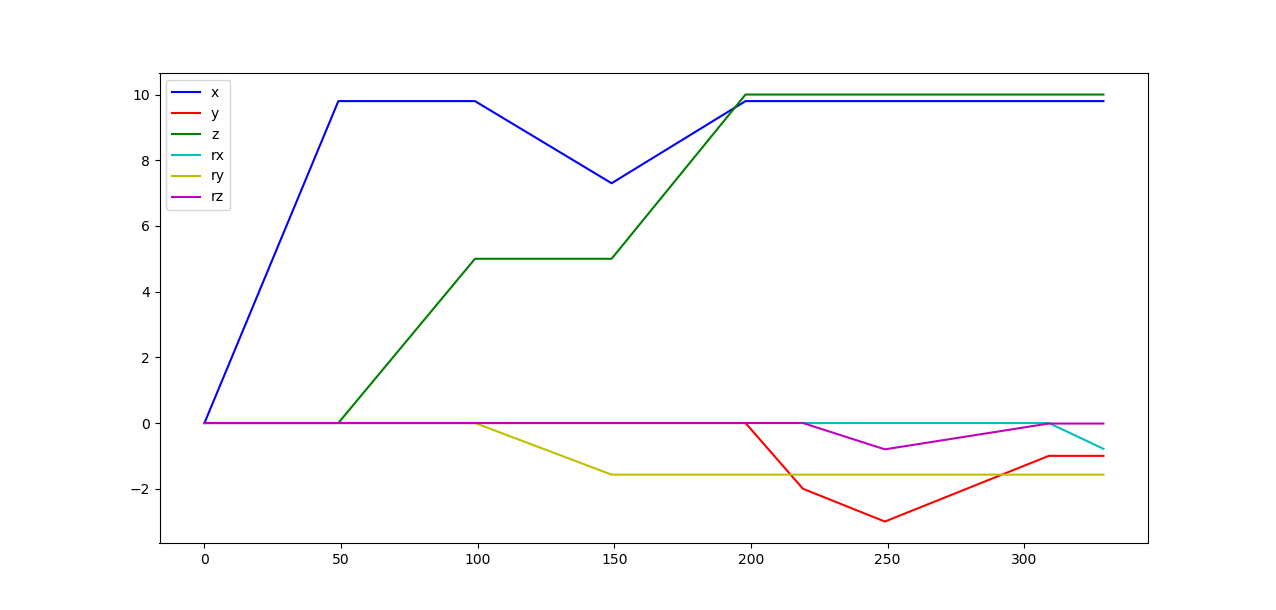
\includegraphics[width=1.0\textwidth]{img/blender_barcelona_traj.png}
  \caption{Blender Barcelona trajectory}\label{fig:blender_barcelona_traj}
\end{figure}

As we see in figure \ref{fig:blender_barcelona_diff} both algorithm struggle for big angle changes without movement. When checking table \ref{tab:barcelona_maximas} and table \ref{tab:barcelona_average} we see that ORB SLAM performs slightly better but with lower frame rate (table \ref{tab:barcelona_fps}) than our SVO SLAM implementation.

\begin{table}[H]
  \centering
  \begin{tabular}{|c|c|c|c|c|c|c|}
  impl & err x & err y & err z & err rx & err ry & err rz\\
  \hline
  Our SVO & 0.622 & 0.537 & 0.956 & 10.417 & 11.222 & 14.682\\
  ORB SLAM& 0.993 & 0.189 & 0.592 & 7.491 & 19.315 & 10.542
\end{tabular}
\caption{Maximum error in meter (x,y,z) and Degrees (rx,ry,rz)}
\label{tab:barcelona_maximas}
\end{table}

\begin{table}[H]
  \centering
  \begin{tabular}{|c|c|c|c|c|c|c|}
    impl & err x & err y & err z & err rx & err ry & err rz\\
    \hline
    Our SVO & 0.396 & 0.166 & 0.451 & 1.012 & 2.753 & 2.446\\
    ORB SLAM & 0.734 & 0.088 & 0.416 & 0.711 & 2.717 & 1.955
  \end{tabular}
\caption{Average error in meter (x,y,z) and Degrees (rx,ry,rz)}
\label{tab:barcelona_average}
\end{table}

\begin{table}[H]
  \centering
  \begin{tabular}{|c|c|}
  impl & FPS\\
  \hline
  Our SVO & 39.56\\
  ORB SLAM & 22.53
\end{tabular}
\caption{Frame rate}
\label{tab:barcelona_fps}
\end{table}


\begin{figure}[H]
  \subfloat[Our implementation]{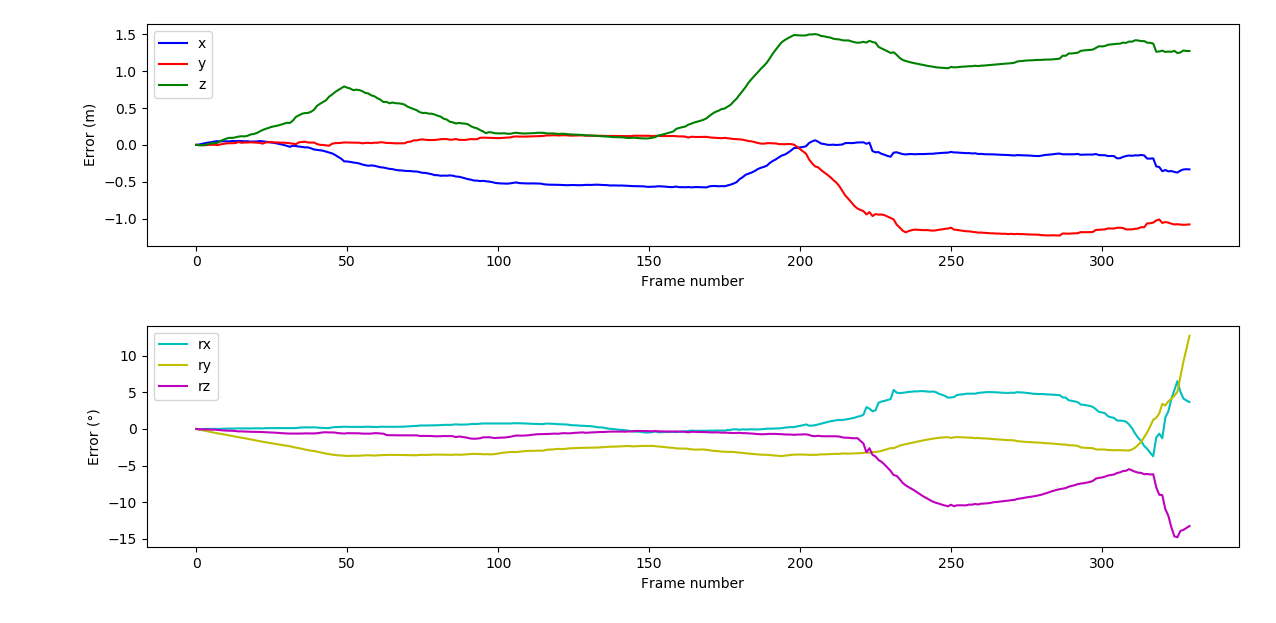
\includegraphics[width=0.9\textwidth]{img/blender_barcelona_our_diff.png}}\\
  \subfloat[ORB SLAM]{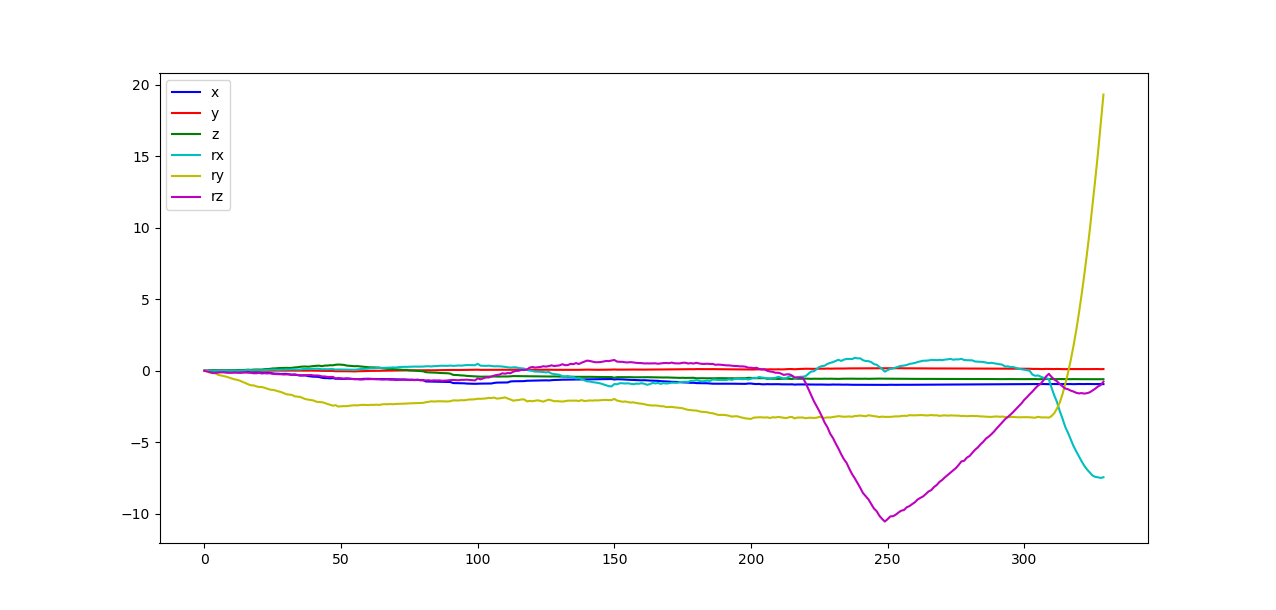
\includegraphics[width=0.9\textwidth]{img/blender_barcelona_orb_diff.png}}
  \caption{Blender Barcelona Scene errors. Distances in meter, angels in Degree.}\label{fig:blender_barcelona_diff}
\end{figure}

\section{EuRoC}

\begin{figure}[H]
  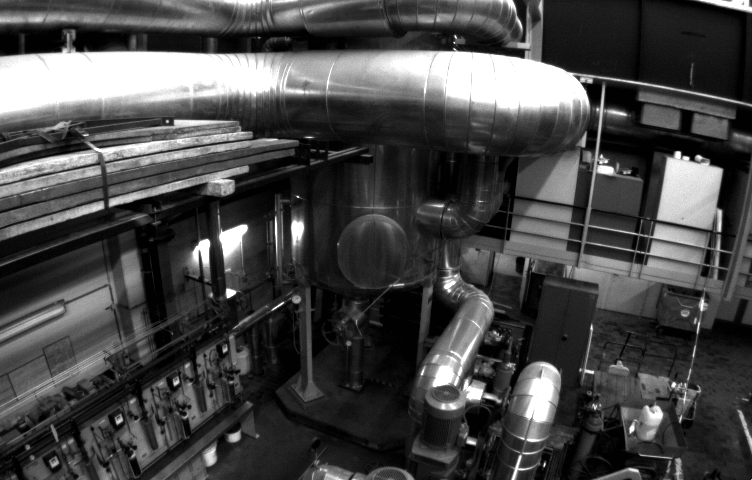
\includegraphics[width=1.0\textwidth]{img/euroc_scene.png}
  \caption{EuRoC Scene}\label{fig:euroc_scene}
\end{figure}

EuRoC is a widely used testset for SLAM algorithms \cite{euroc}. Figure \ref{fig:euroc_scene} shows an image from EuRoC Machine Hall 2. The SVO2 paper \cite{svo2} compares some measurements based on EuRoC. Our measurements are not in the range of any modern SLAM algorithm. However, the problem is that the current implementation doesn't use past keyframes. Therefore, it can't profit if it sees the same scene more than once what increases the drift. For completeness an initial result is shown here for EuRoC Machine Hall 2.

\begin{figure}[H]
  \subfloat[Top View]{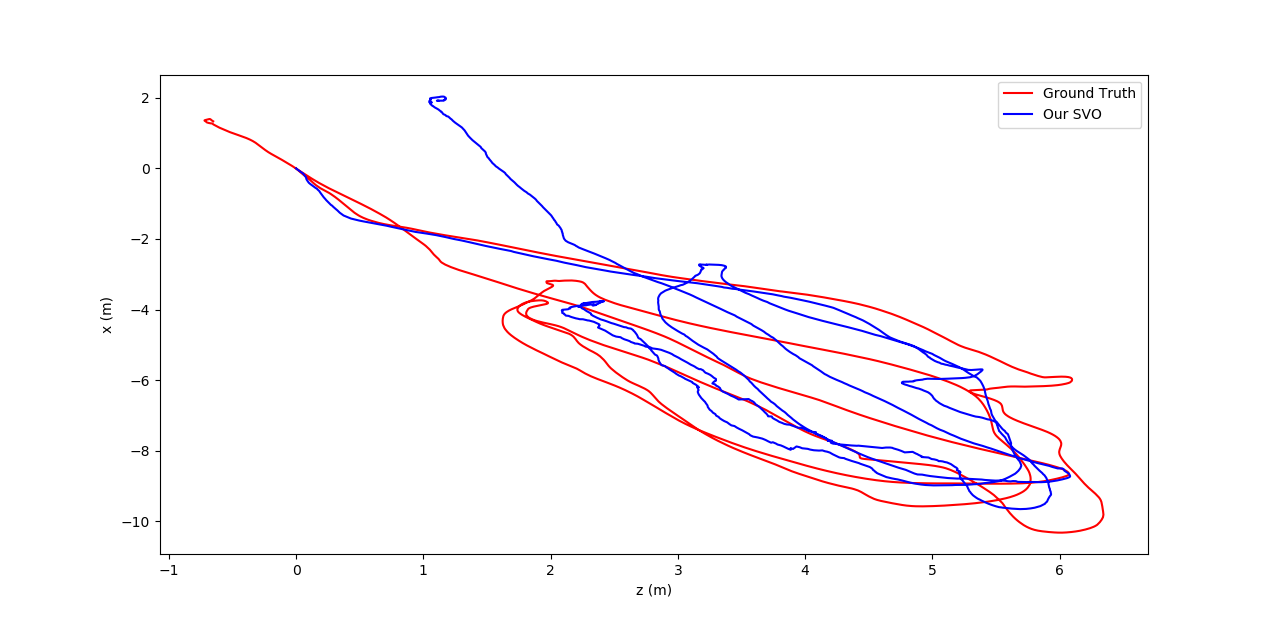
\includegraphics[width=0.9\textwidth]{img/euroc_svo_top.png}}\\
  \subfloat[Side View]{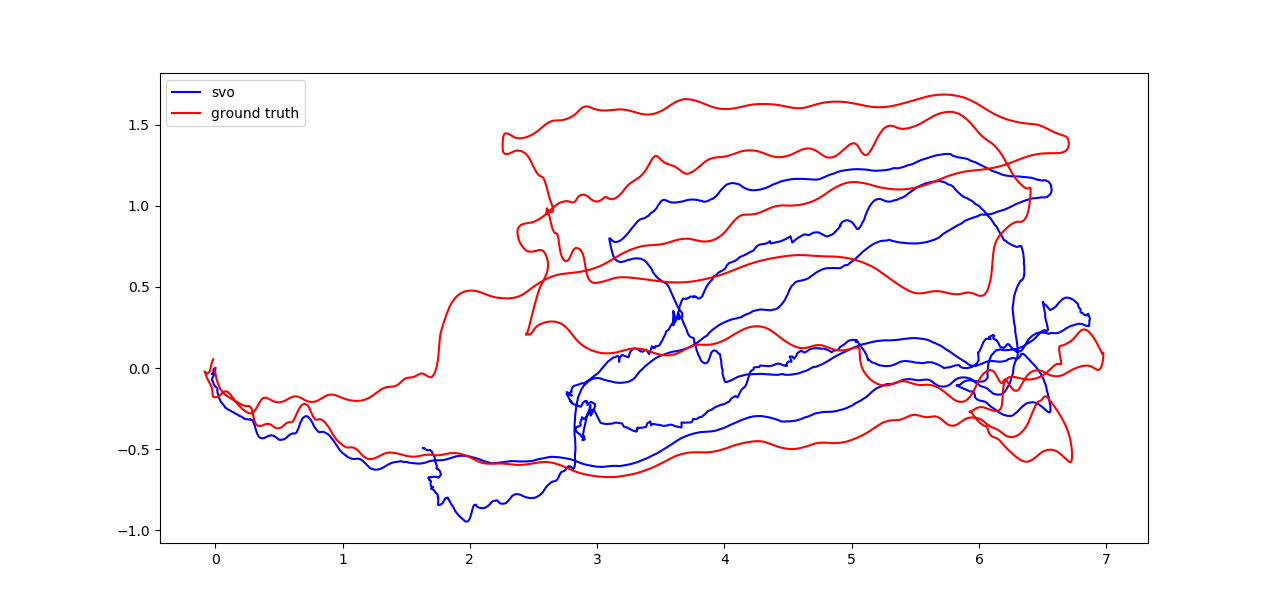
\includegraphics[width=0.9\textwidth]{img/euroc_svo_side.png}}\\
  \caption{EuRoC }\label{fig:euroc}
\end{figure}

As we can see in figure \ref{fig:euroc} we have a huge drift over the whole sequence. In the end we measure an error of more than one meter in each direction. However, this was measured without doing a lot of parameter tuning. SVO2 states that they can achieve an RMSW of only 8 cm. SVO 1 where this thesis is based on can't follow the sequence. It is possible that better results could be achieved with our implementation by tweaking the parameters but it's unrealistic to get close to what SVO2 measured. The average frame rate was 37.13 fps.

\chapter{Discussion}\label{ch:discussion}

We showed that the principle of SVO works and can be faster than e.g. ORB SLAM. Our implementation does not achieve the same frame rate as the reference implementation. There can be a lot of reasons why this happens. First we only use gradient descent for optimization. Probably a Gauss Newton like algorithm would find the minimum faster. We've chosen gradient descent because it is easy understandable and convenient to debug. However, a rework should definitely address this issue. Further we don't use OpenMP. The code is prepared for it but it is no activated because on the test system with an i7 processor the algorithm runs slower. The assumption is that it has to do with optimization and that for some reason the compiler can't vectorize the code when OpenMP is used. On an ARM iMX8QM based system activating OpenMP showed a speedup of around 3. However, even with this speed up the algorithm run with 10fps. Therefore, we did not document this test in more detail. However, two things would be interesting to analyze. Can the compiler vectorize all critical parts of the code and can in parallel enable OpenMP. If we would achieve a speed up of at least 2 with OpenMP frame rates of > 60fps should be achievable.\\\\
The accuracy of our implementation is behind modern SLAM implementations. This could be improved by projection old keypoints into the current frame. We don't do that at the moment because of speed concerns and to keep the algorithm simple. However, it could lead to more stable results because some kind of local loop closing would be possible.\\\\
We implemented a 3D viewer which can be used over a network connection. This approach would allow us to debug devices that are further away e.g. via Wifi or Ethernet. The viewer could be optimized by only asking for differences from the target and not for all keyframes. This would reduce the bandwidth when e.g. using Wifi. However, as a proof of concept this seems to be a good approach.\\\\
We showed an easy way to generate test scenes by using Blender animations. This allows us to make debugging much easier because we know all movements in detail and we can have predefined movements in exactly one direction. Such scenes help debugging algorithms a lot and makes also the comparison of results easy. Generating such scenes is simple, cheap and quick.\\\\
A demo application shows what is possible with SLAM. It is a simple augmented reality application that can be used as a quick demo to show what SLAM can be used for.\\\\
The current library is in the state of a proof of concept. It is far from productive but it shows that SVO works and that it is promising. The implementation showed to be faster than ORB SLAM but it is not as robust yet. The current state could be used as starting point for further development. It is open source and has only dependencies to OpenCV. This makes it much easier to compile it for other platforms like ARM based devices.

\printbibliography

\end{document}
